\begin{apendicesenv}

% Imprime uma página indicando o início dos apêndices
\partapendices

% ----------------------------------------------------------
% ----------------------------------------------------------
% -------------------------------------------------------


\appendix

%\begin{landscape}
%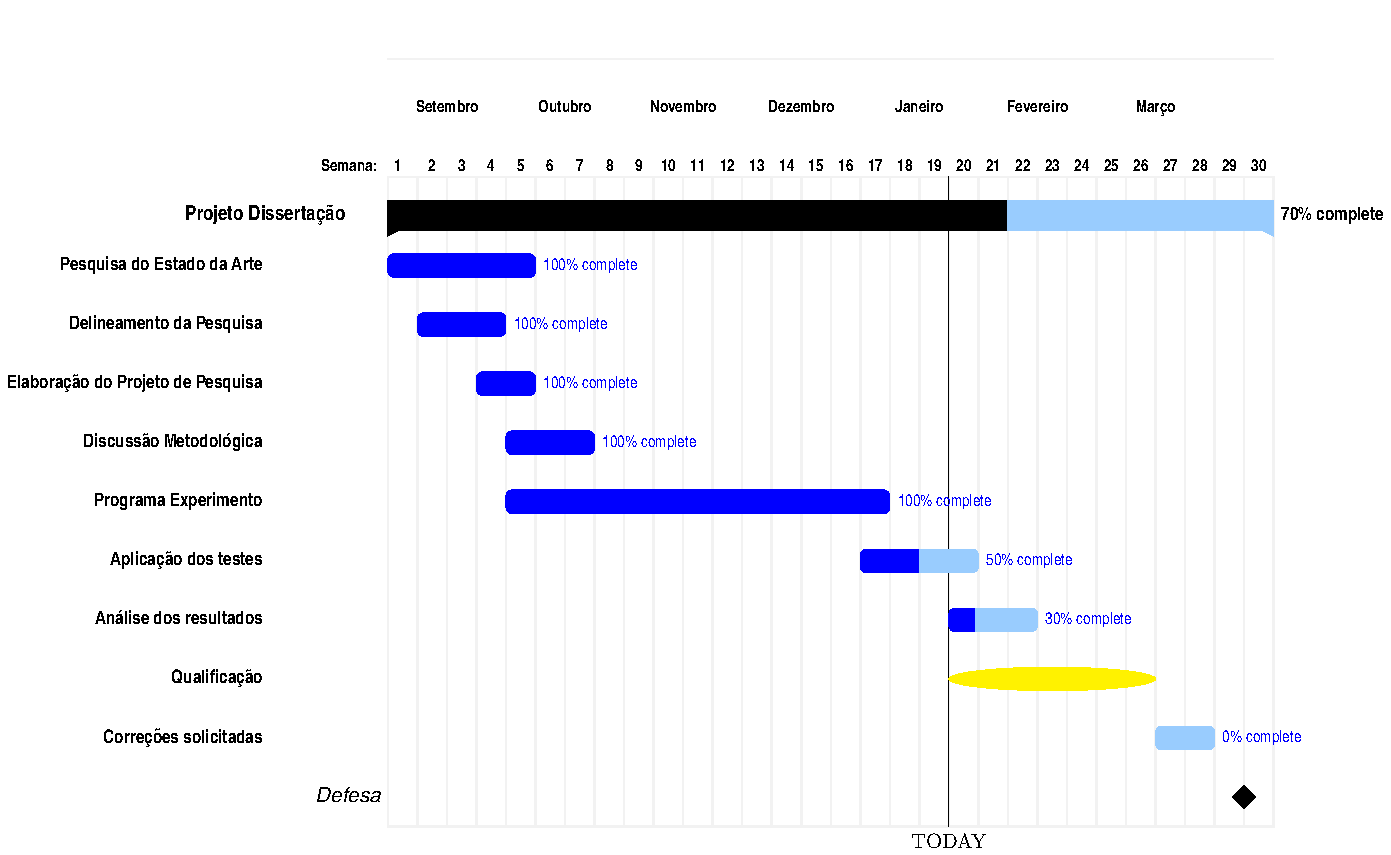
\includepdf[landscape=true,scale=0.87, pagecommand=\chapter{Cronograma}]{apendece/cronograma.pdf}
%\end{landscape}

\chapter{Materiais disponibilizados no aplicativo}
\label{chap:tabela_2}
\begin{longtable}{p{3.5cm}p{11.0cm}}

\caption[\textbf{Materiais disponibilizados no aplicativo}]{\textbf{Conteúdos difundidos pelo aplicativo empreenda agro sustentável}} 
\label{tabela_2} \\

\hline \hline \multicolumn{1}{p{3.5cm}}{\textbf{Base de assuntos}} & \multicolumn{1}{c}{\textbf{Conteúdos}}\\ \hline 

\endfirsthead

\multicolumn{2}{c}%

{{ \bfseries \tablename \ \thetable{} - \ \textbf{Continuação}}}\\

    \hline \multicolumn{1}{p{3.5cm}}{\textbf{Métodos, Técnicas e Recursos}} & \multicolumn{1}{c}{\textbf{Aplicações}}  \\ \hline 

\endhead

\hline \multicolumn{2}{r}{{\textbf{Continua}}} \\ \hline

\endfoot
\hline \multicolumn{2}{r}{{\textbf{Continua}}} \\ \hline

\endfoot
\hline \multicolumn{2}{r}{{\textbf{Conclusão}}} \\ \hline
\hline \hline

\endlastfoot

Conceitos Básicos de Ideação & Insights; Startup Enxuta: Visão, direção e aceleração; Design thinking: Preparação, Ideação I, II e II, finalizando a descoberta \cite{alt_design_2018}. \\

Conceitos Básicos de modelo de negócio (CANVAS) & Briefing, seguimentos de clientes, proposta de valor, canais, relacionamento com clientes e fontes de Receitas, atividades-Chave e estrutura de Custo. \cite{finocchio_junior_project_2013} \\

Conceitos Básicos de Gestão ágil & Gerência do projeto ágil, manifesto Ágil: liderança e organização com Uscrum, início, planejamento e execução do projeto com Agile; Revisão, retrospectiva e encerramento de projetos com Agile, \cite{abrahamsson_agile_2017}. \\ 

Conceitos Básicos da Marketing & Marketing pessoal; Marketing digital/e-commerce: E-mail Marketing: Segmentação ao AB, introdução aos canais não pagos; Google Analytics; Shopify e Inteligência comercial. \cite{ritossa_marketing_2009, rizzo_marketing_2017}. \\ 

Conceitos Básicos da Marketing
Conceitos Básicos de Propriedade Intelectual
 & Direito autoral, Propriedade Industrial e Proteção Sui Generis, \cite{wipo_guide_2019} \\ 

\end{longtable}
\fonte{O autor}

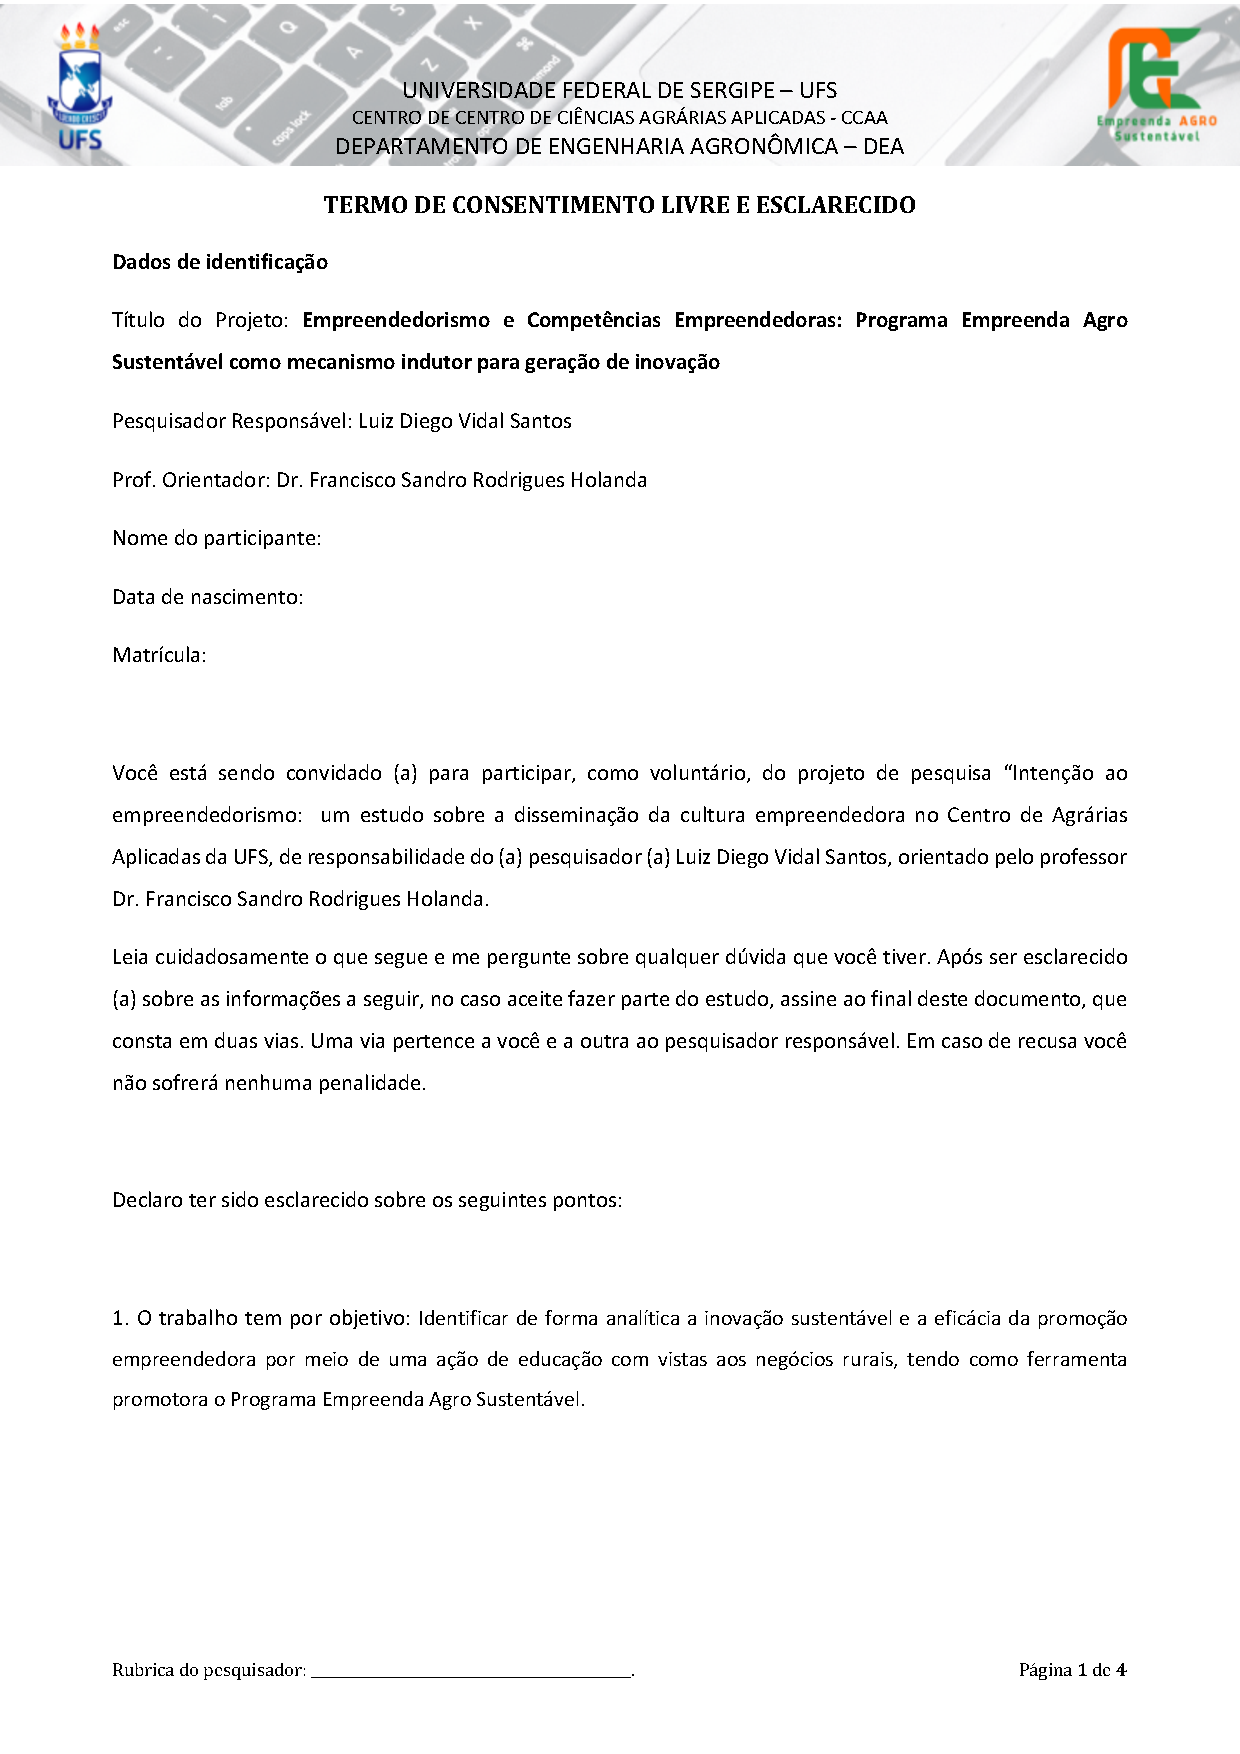
\includepdf[scale=0.80,pagecommand=\chapter{Termo de Consentimento Livre e Esclarecido TCLE}]{apendece/Termo.pdf}


%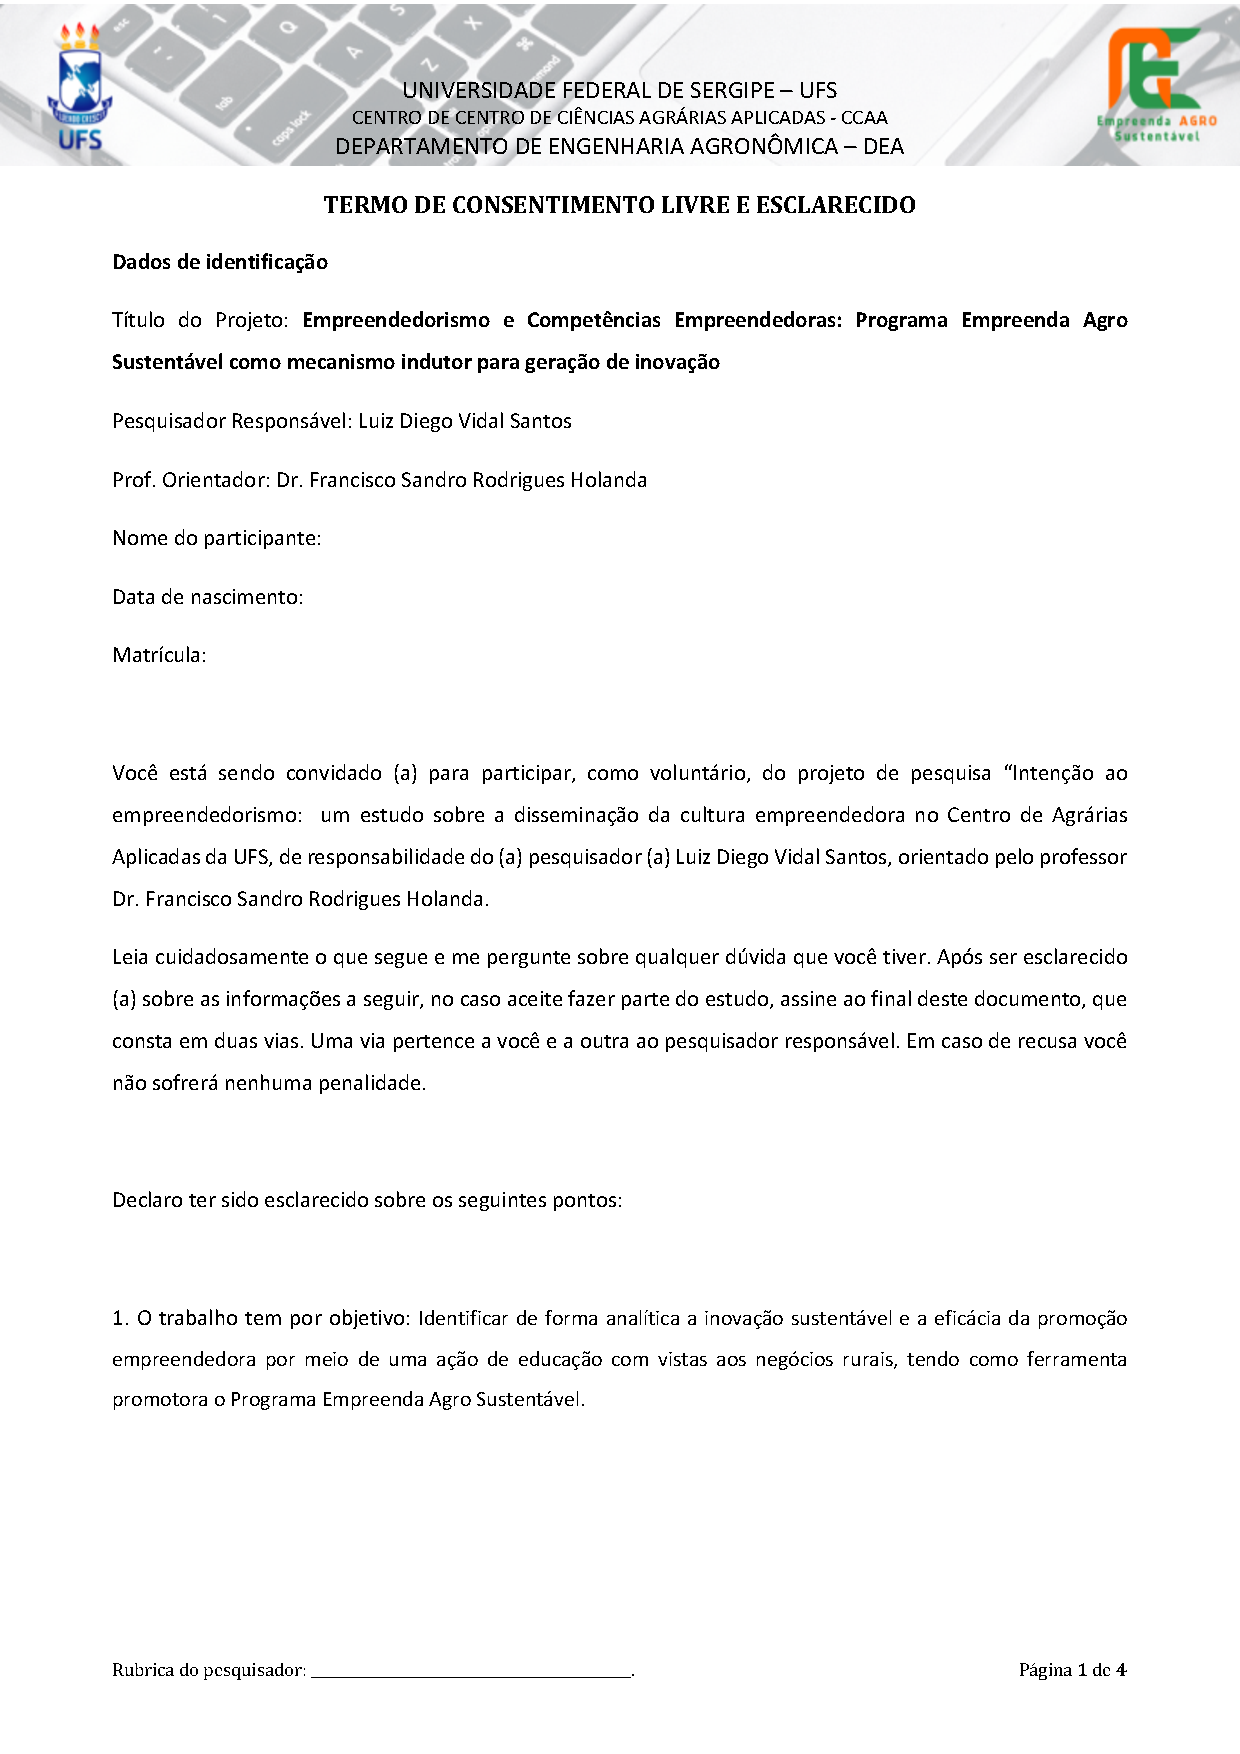
\includepdf[scale=0.87, pagecommand=\chapter{Termo de Consentimento Livre e Esclarecido TCLE}]{apendece/Termo.pdf}


\chapter{Estrutura fatorial da medida de intenção empreendedora}
\label{chap:tabela_3}

\begin{longtable}[H]{p{6cm} c c c }
\caption{\textbf{Estrutura fatorial da medida de intenção empreendedora}}
\label{tabela_3}\\
\hline \hline
\multicolumn{1}{p{6cm}}{} & \multicolumn{3}{c}{\textbf{Fatores}}\\ 
 \multicolumn{1}{c}{\textbf{Itens}} & \multicolumn{3}{c}{\hrulefill}\\ 

 \multicolumn{1}{c}{} 
 &\multicolumn{1}{p{1.5cm}}{\textbf{Autoeficácia}} & \multicolumn{1}{p{1.5cm}}{\textbf{Intenção}} &\multicolumn{1}{p{1.5cm}}{\textbf{Família}}  
\\ \hline 

\endfirsthead

\multicolumn{4}{l}{{{\bfseries \tablename \ \thetable{} -\ \textbf{Estrutura fatorial da medida de intenção empreendedora}}}}\\
\multicolumn{4}{r}{\bfseries \textbf{(continuação)}}\\

\hline \multicolumn{1}{p{6cm}}{\textbf{Questões}} &\multicolumn{1}{c}{\textbf{Autoeficácia}} & \multicolumn{1}{c}{\textbf{Intenção}} &\multicolumn{1}{c}{\textbf{Família}}  
\\ \hline 

\endhead

\hline \multicolumn{4}{r}{\textbf{(Continua)}} \\ \hline


\endfoot
\hline \multicolumn{4}{r}{\textbf{(Conclusão)}} \\ \hline
\hline \hline

\endlastfoot

Estabelecer e atingir metas e objetivos
 &  ,752 & & \\\\
 
Gerar novas ideias
 &  ,702 & & \\\\
 
Desenvolver novos produtos
 &  ,772 & & \\\\
 
Fazer análises financeiras
 &  ,547 & & \\\\
 
Reduzir riscos e incertezas
 &  ,683 &  & \\\\
 
Assumir riscos calculados
 &   ,463 & \textbf{,451} & \\\\
 
Tomar decisões em situações de risco
 &   ,522 & & \\\\
 
Administrar o tempo estabelecendo metas
 &   ,649 & & \\\\
 
Responsabilizar-me por ideias e decisões
 & ,456 & &  \\\\
 
Começar minha própria empresa
& ,603 & \textbf{,435}  & \\\\

Conduzir minha própria empresa ao sucesso
 & ,658 & \textbf{,470}  & \\\\
Eu já sou meu próprio patrão na empresa que eu fundei
 & & ,430 &  \\\\

Para mim, ser um empreendedor implica em mais vantagens do que desvantagens
 &  & ,727  & \\\\
 
Uma carreira como empreendedor é atrativa
 &  & ,890  & \\\\
 
Se tivesse a oportunidade e os recursos, eu me tornaria um empreendedor
 &  & ,788 & \\\\
 
Ser um empreendedor traria grande satisfação
 &  & ,821 & \\\\
 
Por gentileza, indique quão seriamente tem pensado em criar seu próprio negócio
 &  & ,588 & \\\\
 
O capital oferecido por minha família e empréstimo em condições flexíveis são facilitadas
 &  & & ,618 \\\\
 
Minha família me fornece contatos com pessoas que podem me ajudar na carreira de empreendedor
 &  & & ,658 \\\\
 
Minha família me apresenta pessoas de sua rede de relação de negócios
 &  & & ,400 \\\\
 
Minha família me transmite conhecimentos ligados ao meu setor de atividade
 &  & & ,618 \\\\
 
Meus pais / minha família são meus mentores ou \textit{coachs} nas minhas atividades de empreendedor
 &  & & ,687 \\\\
 
Minha família me fornece locais/ infraestrutura para minhas atividades de empreendedor.
 &  & & ,658 \\\\
 
Meus pais ou família me concedem acesso a uma rede de distribuição para minha empresa.
 &  & & ,702 \\\\
 
 
Minha família me empresta capital que  tenho que pagar regularmente a eles com juros		
 &  & & ,583 \\\\
 
Minha família me empresta capital sem a necessidade de juros e que pode ser perdido se o negócio falir
 & & & ,556 \\\\ \hline 
 
\end{longtable}
\fonte{O Autor}
\footnotetext[1]{Método de Extração: Análise de Componente Principal.\\Método de Rotação: Varimax com Normalização de Kaiser.}

\chapter{Teste de amostras independentes para as questões relacionadas a autoeficácia}
\label{tab:amostras_autoeficacia}


\begin{longtable}[H]{p{7cm}ccccc}
\caption{\textbf{Teste de amostras independentes para as questões relacionadas a autoeficácia}}
\label{tabela_5}\\
\hline \hline
 &
  \multicolumn{1}{l}{} &
  \multicolumn{1}{l}{} &
  \multicolumn{1}{l}{} &
  \multicolumn{1}{l}{} &
  \multicolumn{1}{l}{} \\
\endfirsthead
%
\multicolumn{6}{c}
{{Tabela \thetable\ - Teste de amostras independentes}} \\
\multicolumn{6}{r}{\textbf{(Continuação)}}
\\ \hline
%
\endhead
%
\endfoot
\hline \multicolumn{6}{r}{\textbf{(Conclusão)}} \\
\hline \hline

\endlastfoot
%
\multicolumn{1}{c}{\textbf{Teste de amostras independentes}} &
  \multicolumn{2}{c}{\textbf{Mediana}} &
  \multicolumn{2}{c}{\textbf{Posto Médio}} &
  \multicolumn{1}{c}{\textbf{\textit{P-value}}} \\ \cline{2-6}
 &
  \textbf{antes} &
  \multicolumn{1}{l}{\textbf{após}} &
  \textbf{antes} &
  \textbf{após} &
  \multicolumn{1}{l}{} \\ \hline
Estabelecer e atingir metas e objetivos &
  5 &
  6 &
  65,36 &
  75,94 &
  0,114 \\
Gerar novas ideias &
  6 &
  6 &
  65,27 &
  76,07 &
  0,110 \\
Desenvolver novos produtos & %Falta fazer
  4 &
  6 &
  61,13 &
  76,06 &
  0,950 \\
Fazer análises financeiras &
  4 &
  6 &
  61,13 &
  76,06 &
  \textbf{0,002} \\
Reduzir riscos e incertezas &
  3 &
  5 &
  58,69 &
  86,31 &
  \textbf{0,000} \\
Assumir riscos calculados &
  4 &
  5 &
  63,08 &
  79,49 &
  \textbf{0,016} \\
Tomar decisões em situações de risco &
  5 &
  5 &
  69,55 &
  69,43 &
  0,986 \\
Administrar o tempo estabelecendo metas &
  5 &
  6 &
  63,50 &
  78,83 &
  \textbf{0,023} \\
Responsabilizar-me por ideias e decisões &
  5 &
  6 &
  64,41 &
  77,42 &
  0,053 \\\hline \hline
\end{longtable}
\fonte{O Autor}

\chapter{Testes de amostras independentes para Participação Familiar e influência de terceiros}
\label{tab:amostras_familiar}

\begin{longtable}[!h]{p{7cm}ccccc}
\caption{\textbf{Testes de amostras dependentes para Participação familiar e influência de terceiros}}
\label{tabela_familair}\\
\hline \hline
 &
  \multicolumn{1}{l}{} &
  \multicolumn{1}{l}{} &
  \multicolumn{1}{l}{} &
  \multicolumn{1}{l}{} &
  \multicolumn{1}{l}{} \\
\endfirsthead
%
\multicolumn{6}{c}
{{Tabela \thetable\ - Testes de amostras independentes para Participação familiar e influência de terceiros}} \\
\multicolumn{6}{r}{\textbf{(Continuação)}}
\\ \hline
%
\endhead
%
\endfoot
\hline \multicolumn{6}{r}{\textbf{(Conclusão)}} \\
\hline \hline

\endlastfoot
%
\multicolumn{1}{c}{\textbf{Teste de amostras independentes}} &
  \multicolumn{2}{c}{\textbf{Mediana}} &
  \multicolumn{2}{c}{\textbf{P. Médio}} &
  \multicolumn{1}{c}{\textbf{\textit{P-value}}} \\ \cline{2-5}
 &
  \textbf{antes} &
  \multicolumn{1}{l}{\textbf{após}} &
  \textbf{antes} &
  \textbf{após} &
  \multicolumn{1}{l}{} \\ \hline
O capital oferecido por minha família é um empréstimo em condições flexíveis e facilitadas (p. ex.: baixas taxas de juros) &
  2 &
  1 &
  73,12 &
  62,67 &
    0,104 \\
Minha família me apresenta pessoas de sua rede de relação de negócios, oferecendo me contato com possíveis parceiros e/ou clientes &
  3 &
  1 &
  74,66 &
  60,31 &
 \textbf{0,030} \\
Minha família me transmite conhecimentos ligados ao meu setor de atividade sobre como oferecer serviços e como produzir os produtos &
  2 &
  1 &
  72,93 &
  60,61 &
  0,056 \\
Meus pais / minha família são meus mentores ou coachs nas minhas atividades de empreendedor &
  2 &
  1 &
  69,41 &
  65,88 &
  0,079 \\
Minha família me fornece locais/ infraestrutura para minhas atividades de empreendedor &
  2 &
  1 &
  71,96 &
  63,25 &
  0,179 \\
Meus pais/minha família me concedem acesso a uma rede de distribuição para minha empresa &
  1 &
  1 &
  60,30 &
  72,51 &
  \textbf{0,045} \\
Pensando em todos os possíveis recursos que minha família me fornece, eu sou completamente dependente dela para decidir como alocá-los e usá-los &
  3 &
  3 &
  69,99 &
  65,02 &
  0,455 \\
O capital oferecido por minha família é um empréstimo em condições flexíveis e facilitadas &
  1 &
  1 &
  75,01 &
  58,61 &
  0,0808 \\
Minha família me empresta capital que eu tenho que pagar regularmente a eles com juros &
  1 &
  1 &
  69,63 &
  68,03 &
  0,783 \\
Minha família me empresta capital sem a necessidade de sem juros e que pode ser perdido se o negócio falir &
  2 &
  1 &
  72,11 &
  64,21 &
  0,205  \\ \hline \hline
\end{longtable}
\fonte{O Autor}


\chapter{Teste de amostras independentes para Intenção Empreendedora}
\label{tab:amostras_intencao_empreendedora}


\begin{longtable}[!h]{p{7cm}ccccc}
\caption{\textbf{Teste de amostras independentes para Intenção Empreendedora}}
\label{tabela_6}\\
\hline \hline
 &
  \multicolumn{1}{l}{} &
  \multicolumn{1}{l}{} &
  \multicolumn{1}{l}{} &
  \multicolumn{1}{l}{} &
  \multicolumn{1}{l}{} \\
\endfirsthead
%
\multicolumn{6}{c}
{{Tabela \thetable\ - Teste de amostras independentes  para Intenção Empreendedora}} \\
\multicolumn{6}{r}{\textbf{(Continuação)}}
\\ \hline
%
\endhead
%
\endfoot
\hline \multicolumn{6}{r}{\textbf{(Conclusão)}} \\
\hline \hline

\endlastfoot
%
\multicolumn{1}{c}{\textbf{Teste de amostras independentes}} &
  \multicolumn{2}{c}{\textbf{Mediana}} &
  \multicolumn{2}{c}{\textbf{P. Médio}} &
  \multicolumn{1}{c}{\textbf{\textit{P-value}}} \\ \cline{2-5}
 &
  \textbf{antes} &
  \multicolumn{1}{l}{\textbf{após}} &
  \textbf{antes} &
  \textbf{após} &
  \multicolumn{1}{l}{} \\ \hline
Começar minha própria empresa &
  5 &
  6 &
  65,66 &
  75,47 &
    0,151 \\
Conduzir minha própria empresa ao sucesso &
  5 &
  6 &
  65,46 &
  74,51 &
  0,177 \\
Eu já sou meu próprio patrão na empresa que eu fundei &
  1 &
  1 &
  72,76 &
  61,83 &
  0,077 \\
Para mim, ser um empreendedor implica em mais vantagens do que desvantagens &
  6 &
  6 &
  65,00 &
  75,34 &
  0,122 \\
Uma carreira de empreendedor é atrativa para mim &
  6 &
  6,5 &
  65,24 &
  73,60 &
  0,202 \\
Se tivesse oportunidade e os recursos eu me tornaria um empreendedor &
  7 &
  7 &
  60,30 &
  72,51 &
  \textbf{0,045} \\
Ser empreendedor me traria grande satisfação &
  6 &
  7 &
  64,39 &
  76,31 &
  0,069 \\
Por gentileza, indique quão seriamente tem pensado em criar seu próprio negócio &
  6 &
  6 &
  64,96 &
  75,41 &
  0,119 \\
Eu já sou patrão na empresa que criei &
  6 &
  6 &
  72,76 &
  61,83 &
  0,077 \\
Tenho pensado em abrir minha empresa &
  6 &
  6 &
  66,67 &
  72,70 &
  0,377  \\ \hline \hline
\end{longtable}
\fonte{O Autor}

\chapter{Podcast Empreenda Agrocast}
\label{app:poscast}
\begin{figure}[H]
\FloatBarrier
\center
\caption{\textbf{Podcast Empreenda Agrocast}}
\subfigure[ref1][Empreenda Agrocast]{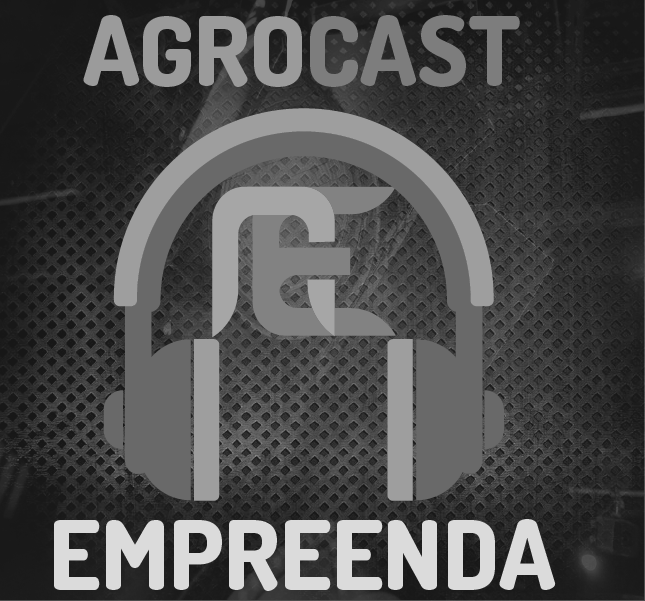
\includegraphics[scale=0.28]{Imagens/podcast_1.png}}
\qquad
\subfigure[ref2][Materiais de apoio produzidos]{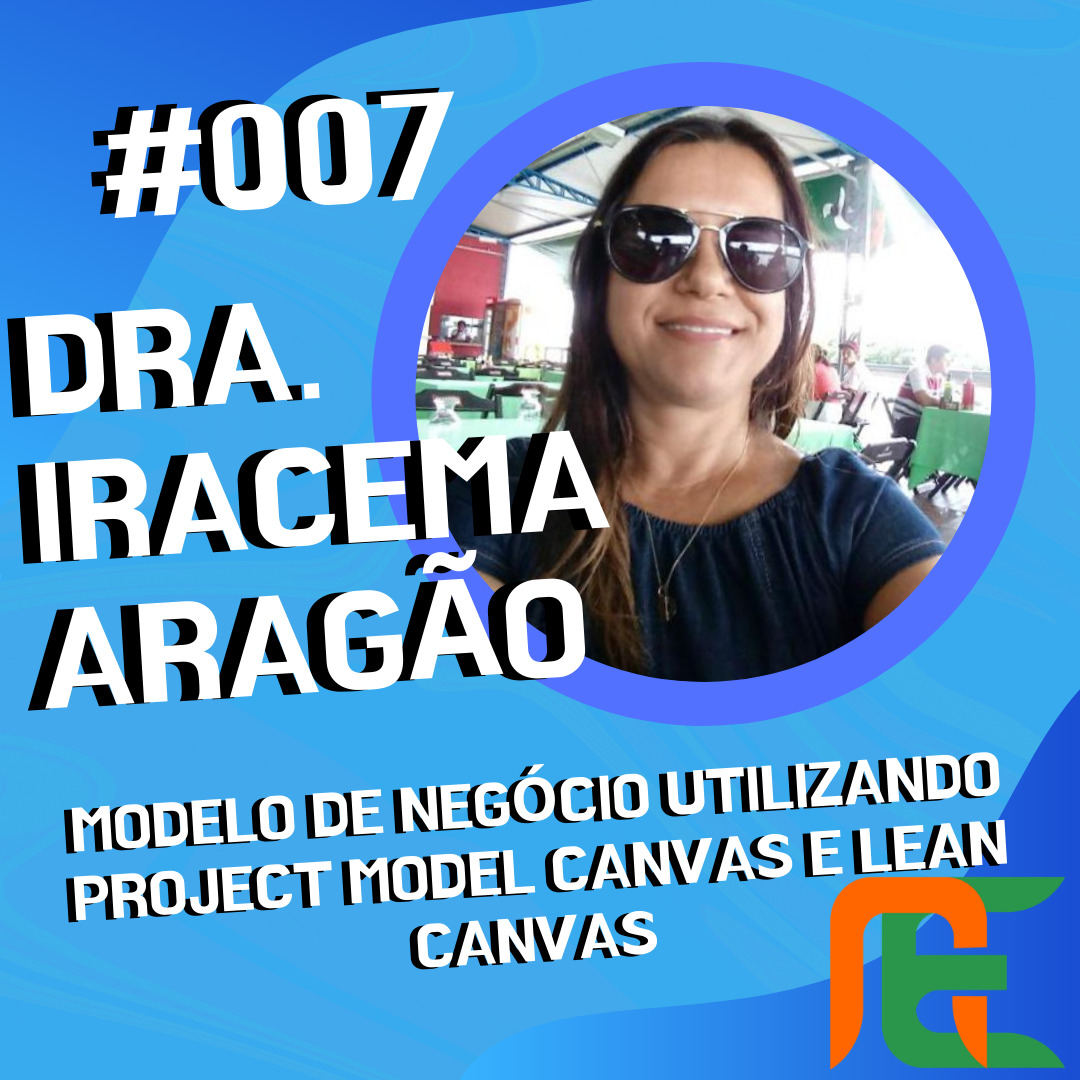
\includegraphics[scale=0.2]{Imagens/podcast_2.jpg}}
\qquad
\subfigure[ref3][Materiais de apoio produzidos]{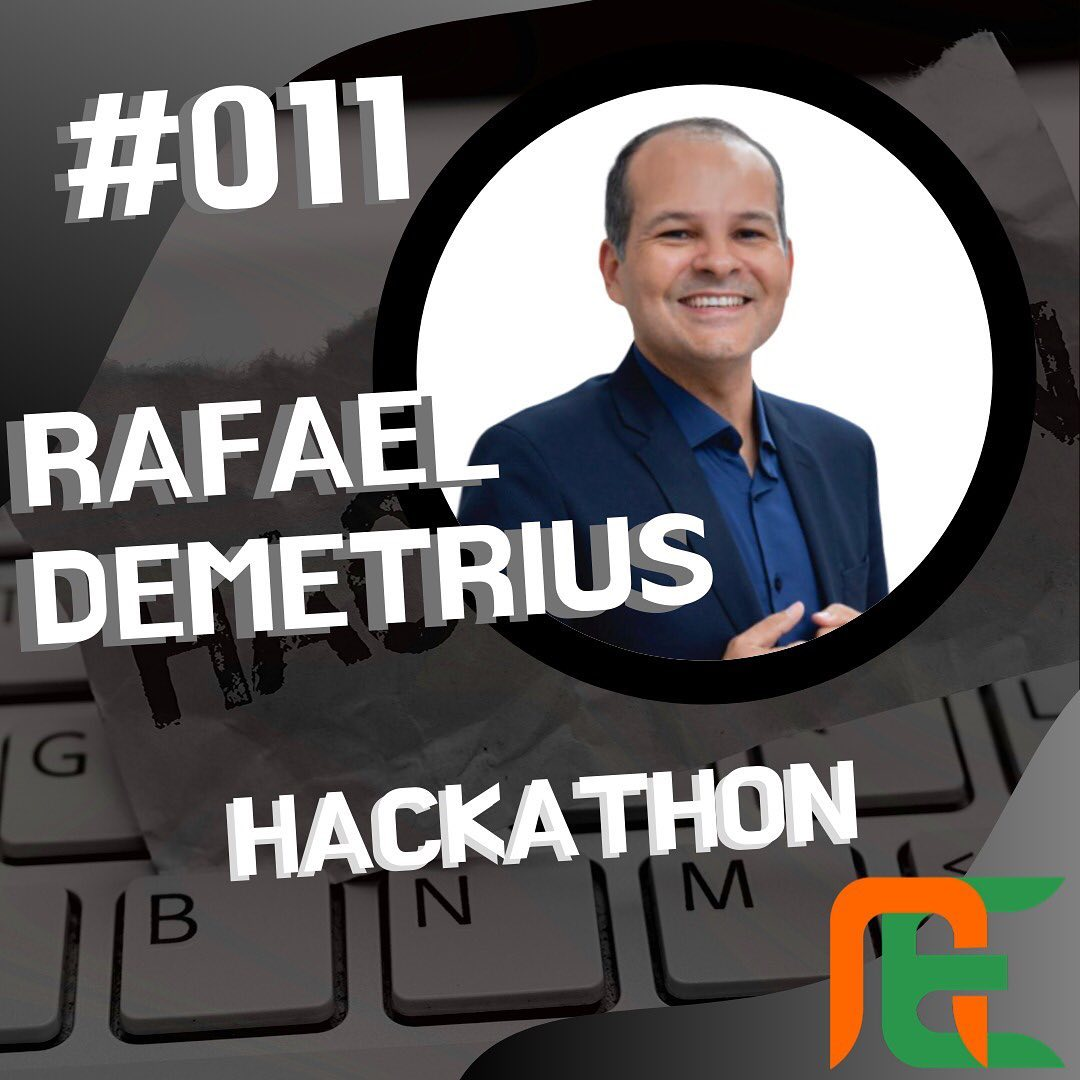
\includegraphics[scale=0.16]{Imagens/podcast_3.jpg}}
\qquad
\subfigure[ref3][Colaborador entrevistado]{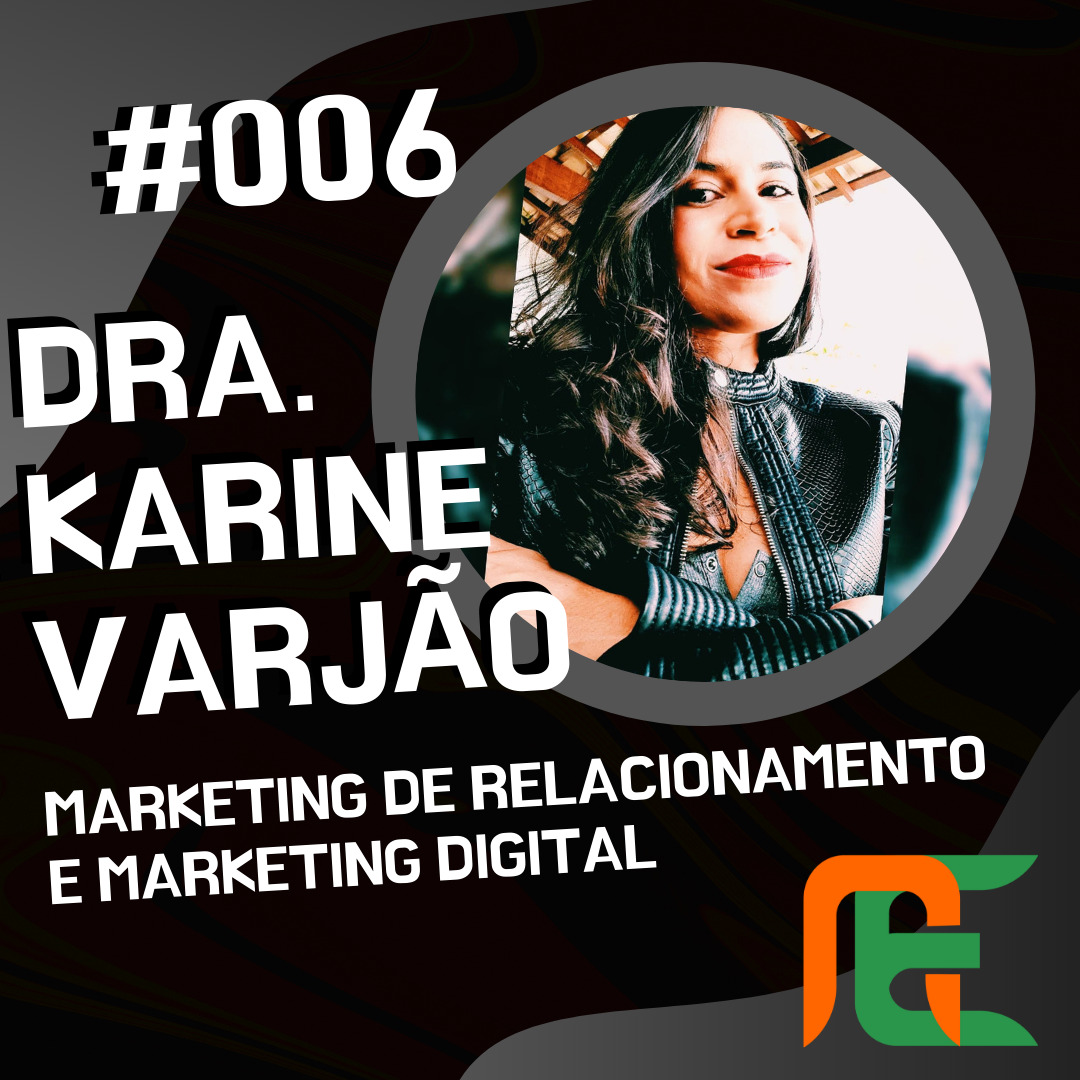
\includegraphics[scale=0.2]{Imagens/podcast_4.jpg}}
\qquad
\subfigure[ref3][Colaborador entrevistado]{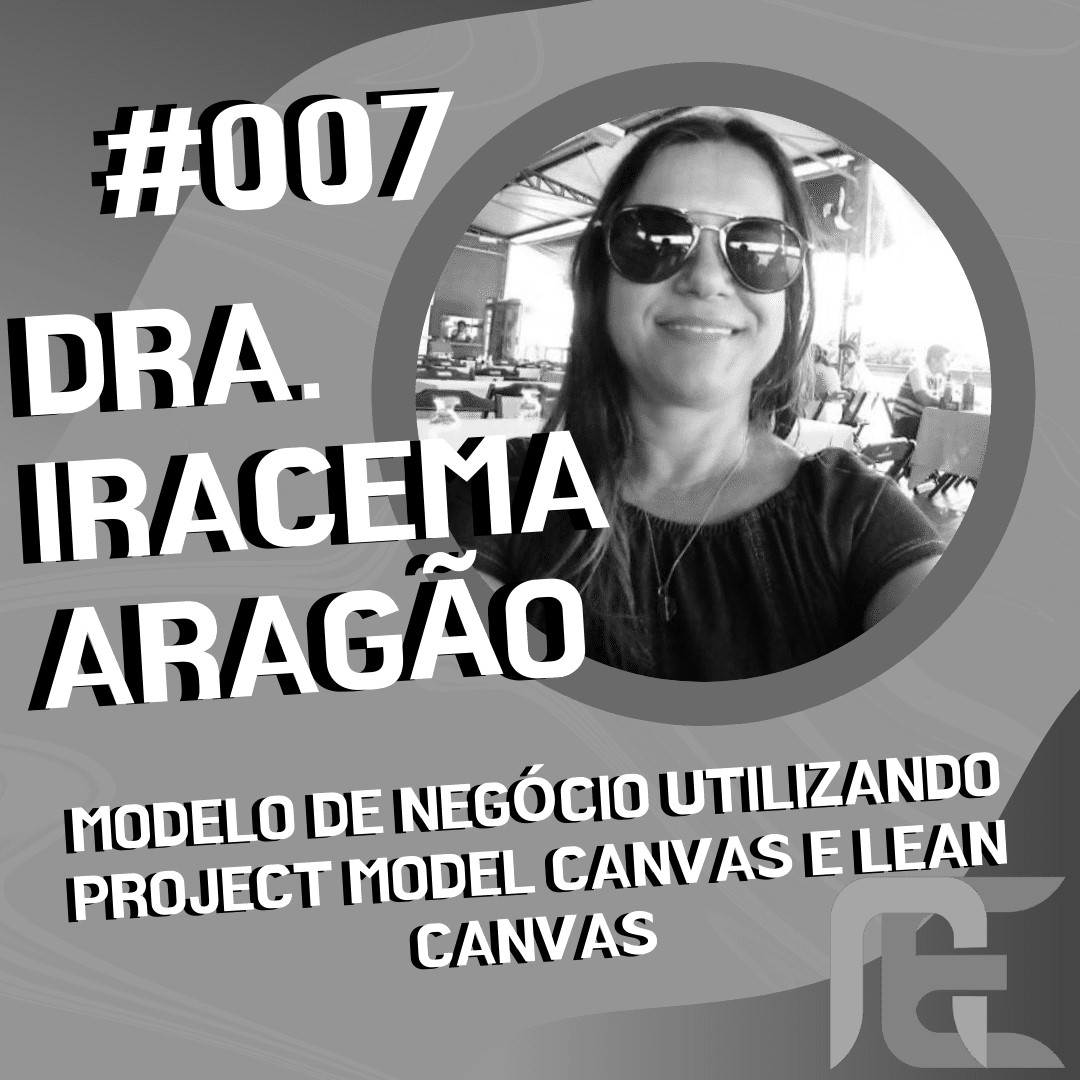
\includegraphics[scale=0.2]{Imagens/podcast_5.jpg}}
\qquad
\subfigure[ref3][Colaborador entrevistado]{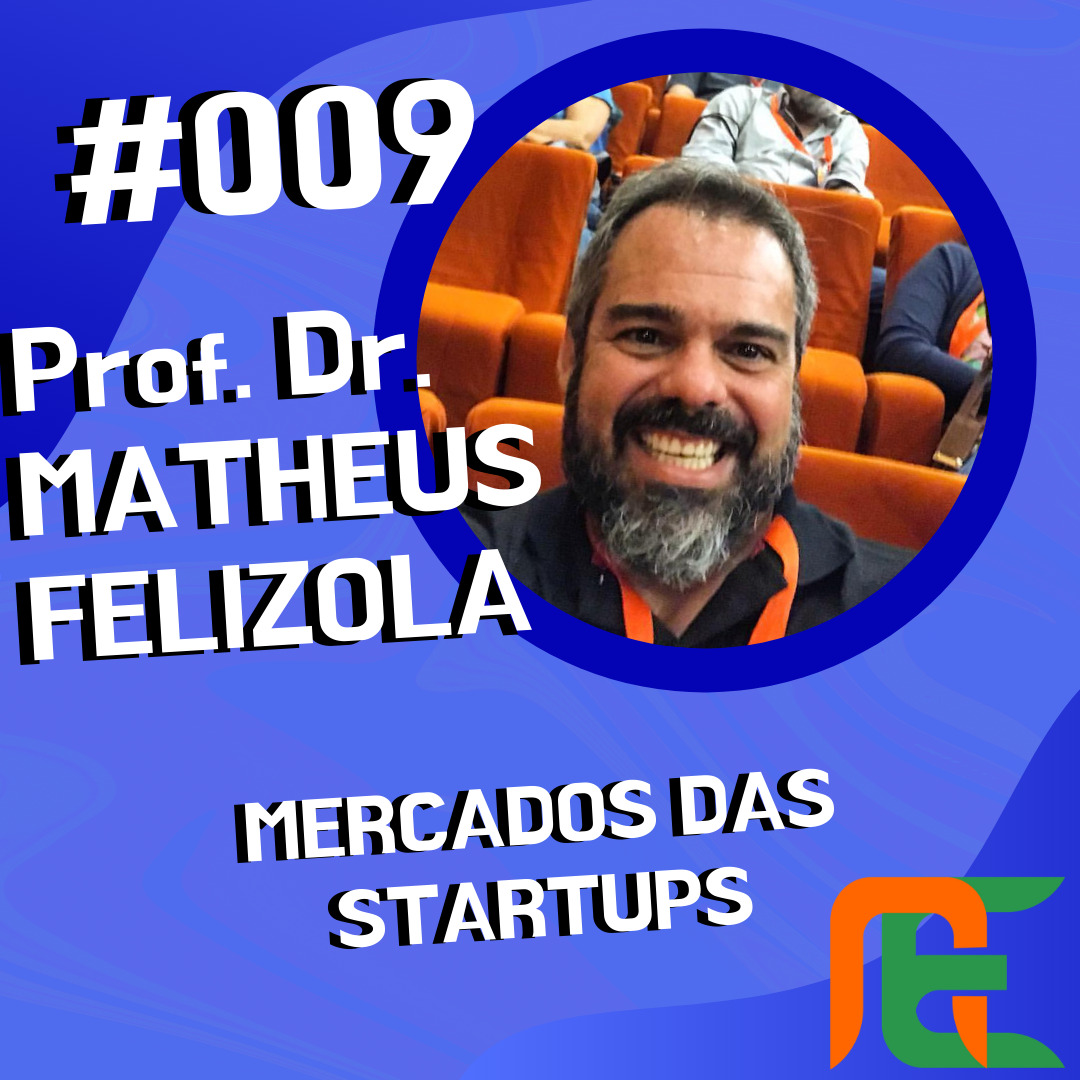
\includegraphics[scale=0.2]{Imagens/podcast_6.jpg}}
\fonte{O Autor}.
\label{figura_podcast}
\end{figure}

\chapter{1º Workshop Empreenda Agro Sustentável}
\label{app:workshop_1}

\begin{figure}[H]
\FloatBarrier
\center
\caption{\textbf{1º Workshop Empreenda Agro Sustentável}}
\subfigure[ref1][Abertura do 1º Workshop ]{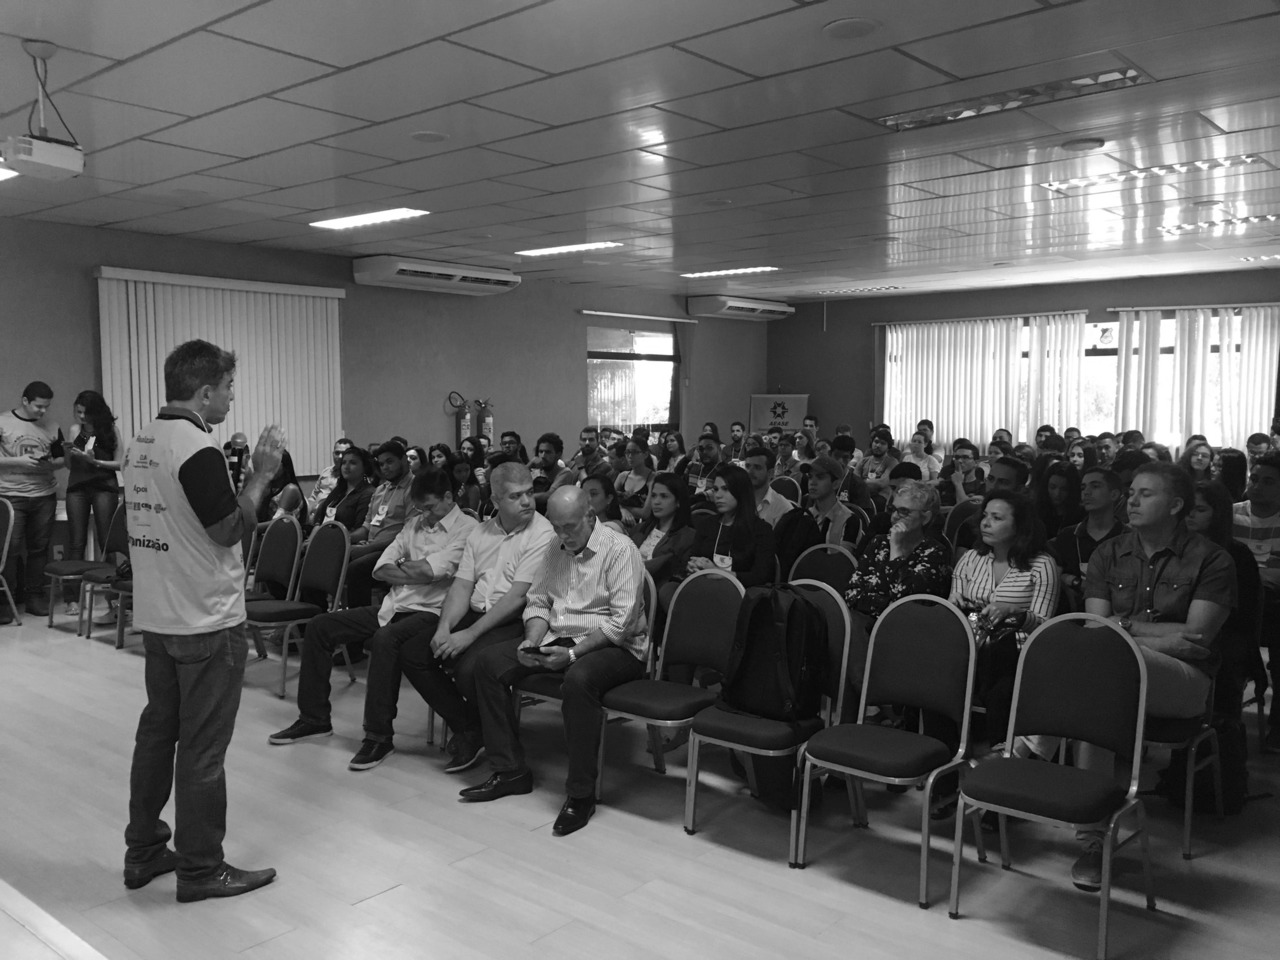
\includegraphics[scale=0.048]{Imagens/primeiro_dia_6.jpg}}
\qquad
\subfigure[ref2][Palestras do programa: 2º dia]{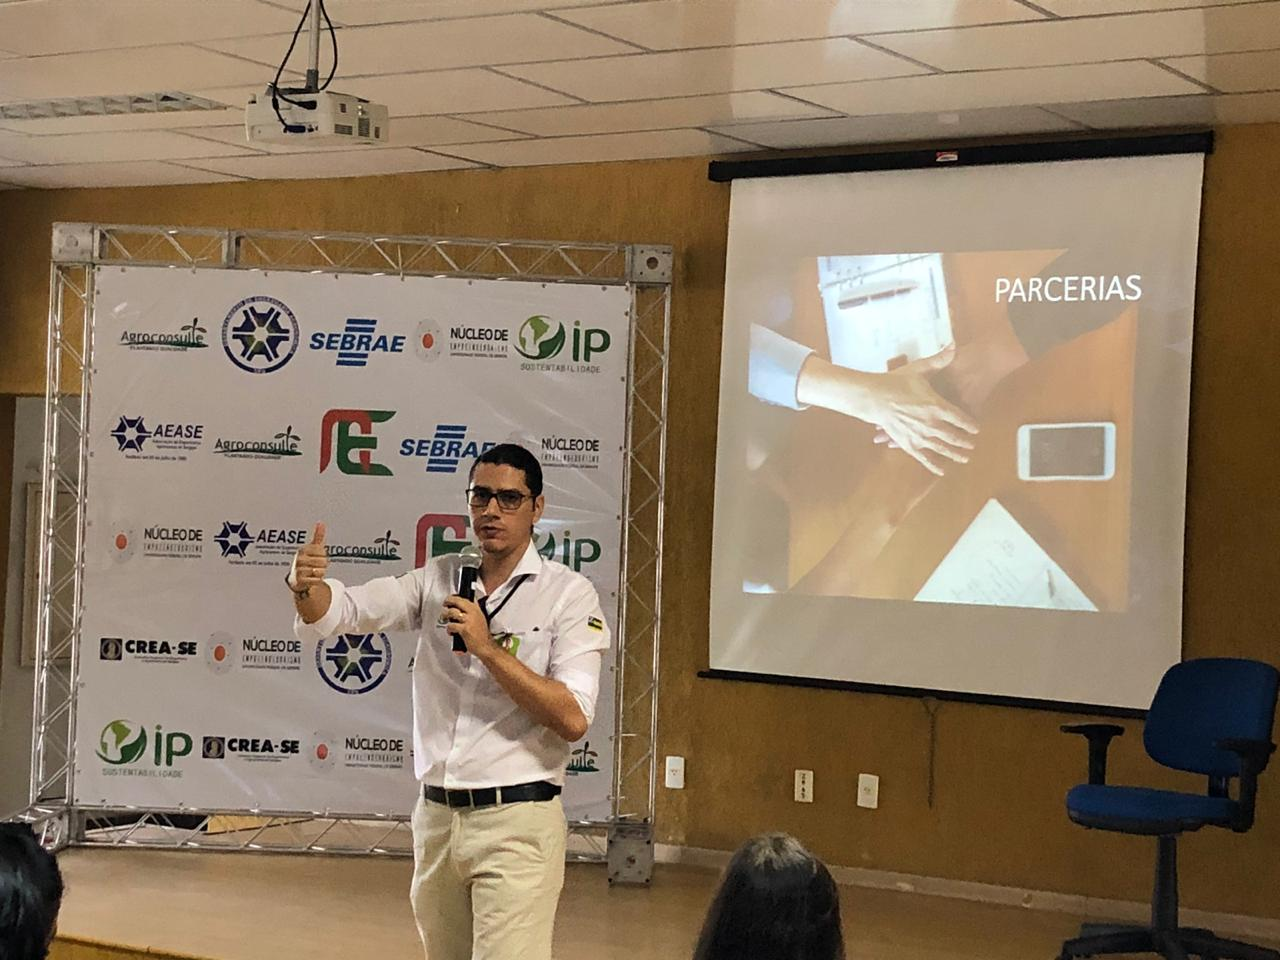
\includegraphics[scale=0.15]{Imagens/primeiro_dia_7.jpg}}
\qquad
\qquad
\subfigure[ref3][Palestras do programa: 2º dia]{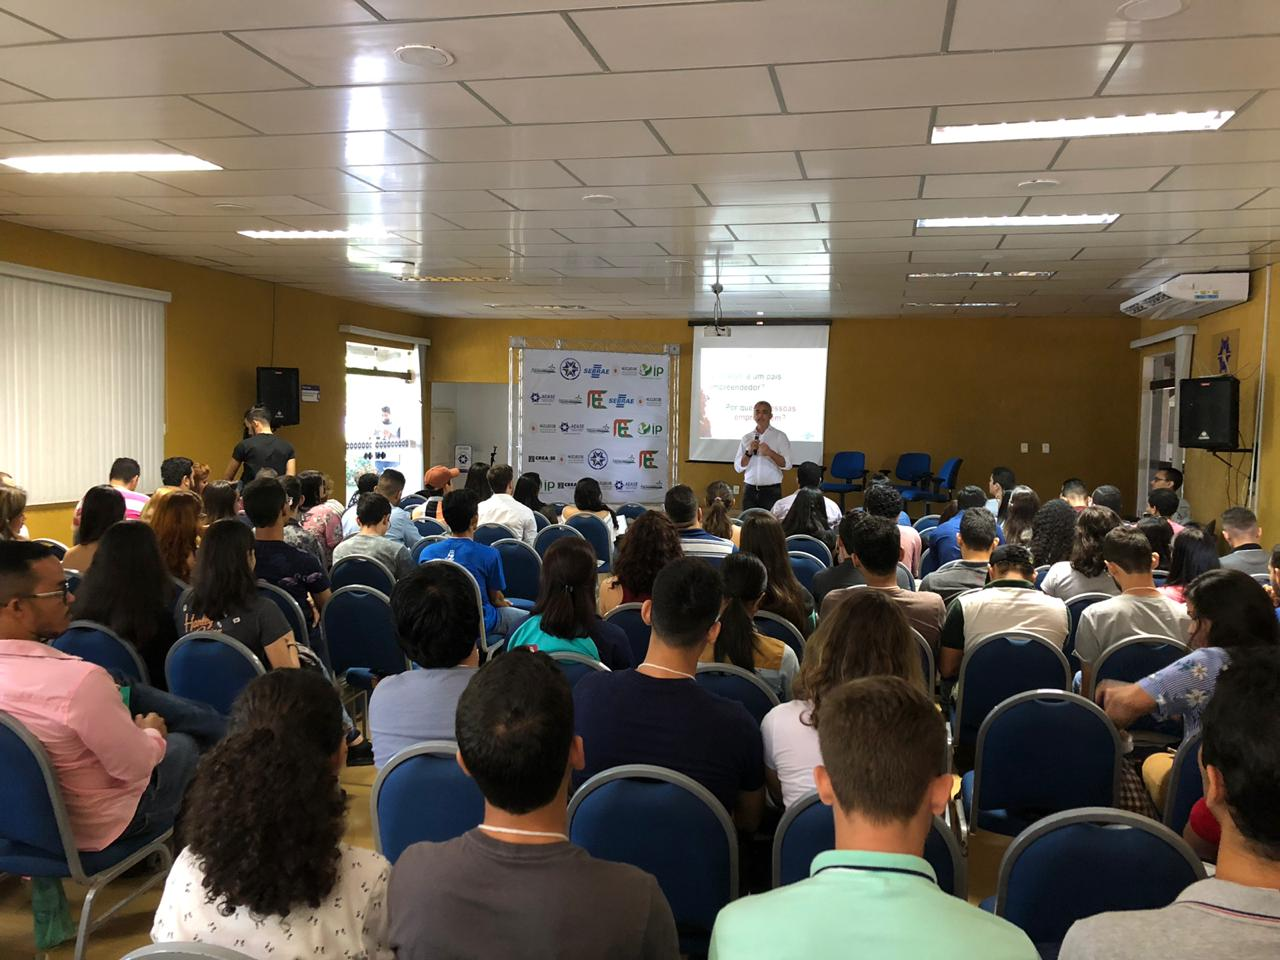
\includegraphics[scale=0.15]{Imagens/primeiro_dia_1.jpg}}
\qquad
\subfigure[ref4][Palestras do programa: 2º dia]{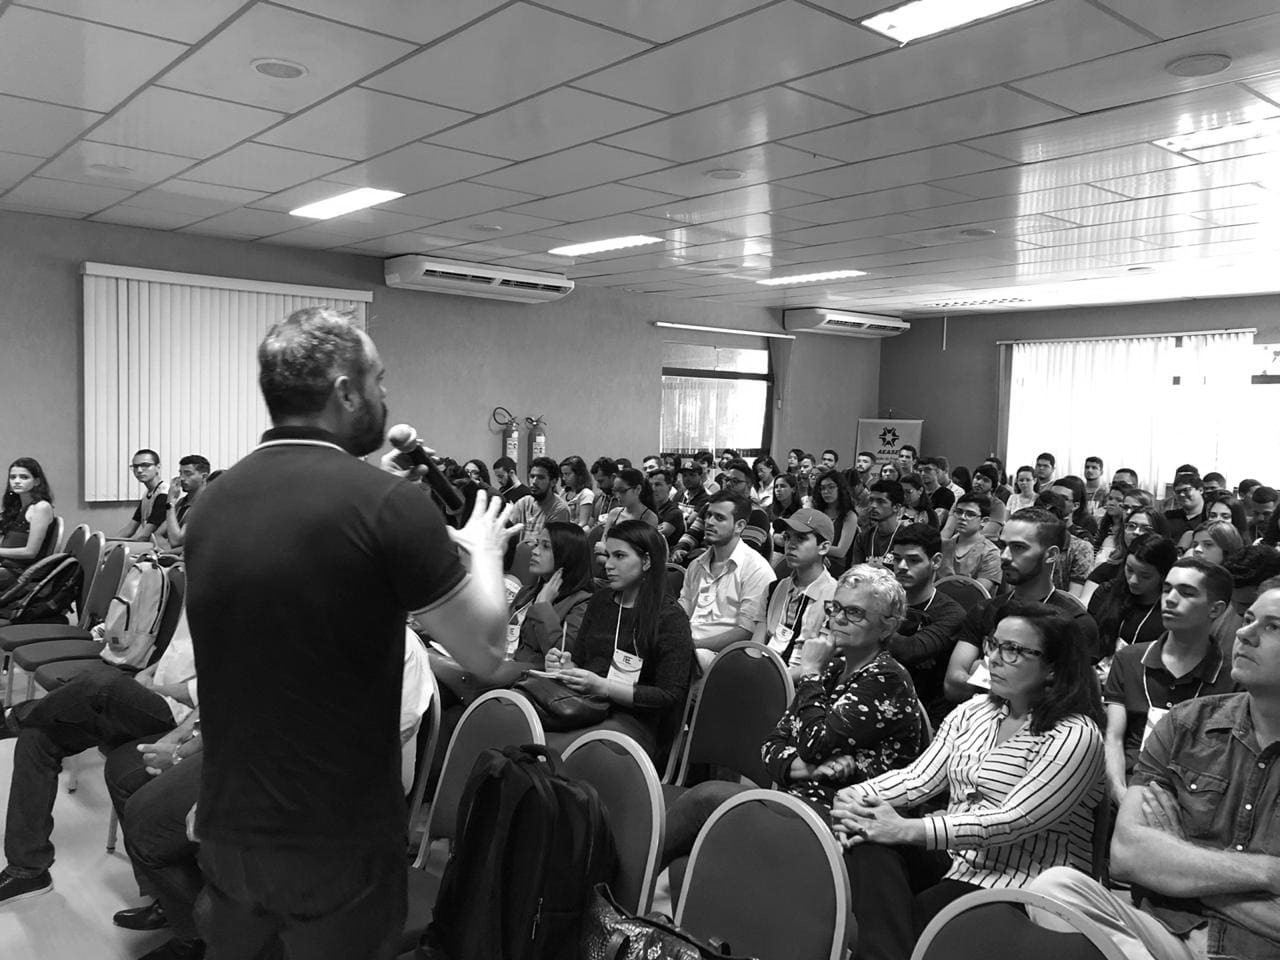
\includegraphics[scale=0.15]{Imagens/primeiro_dia_2.jpg}}
\subfigure[ref5][Participantes do programa: 2º dia]{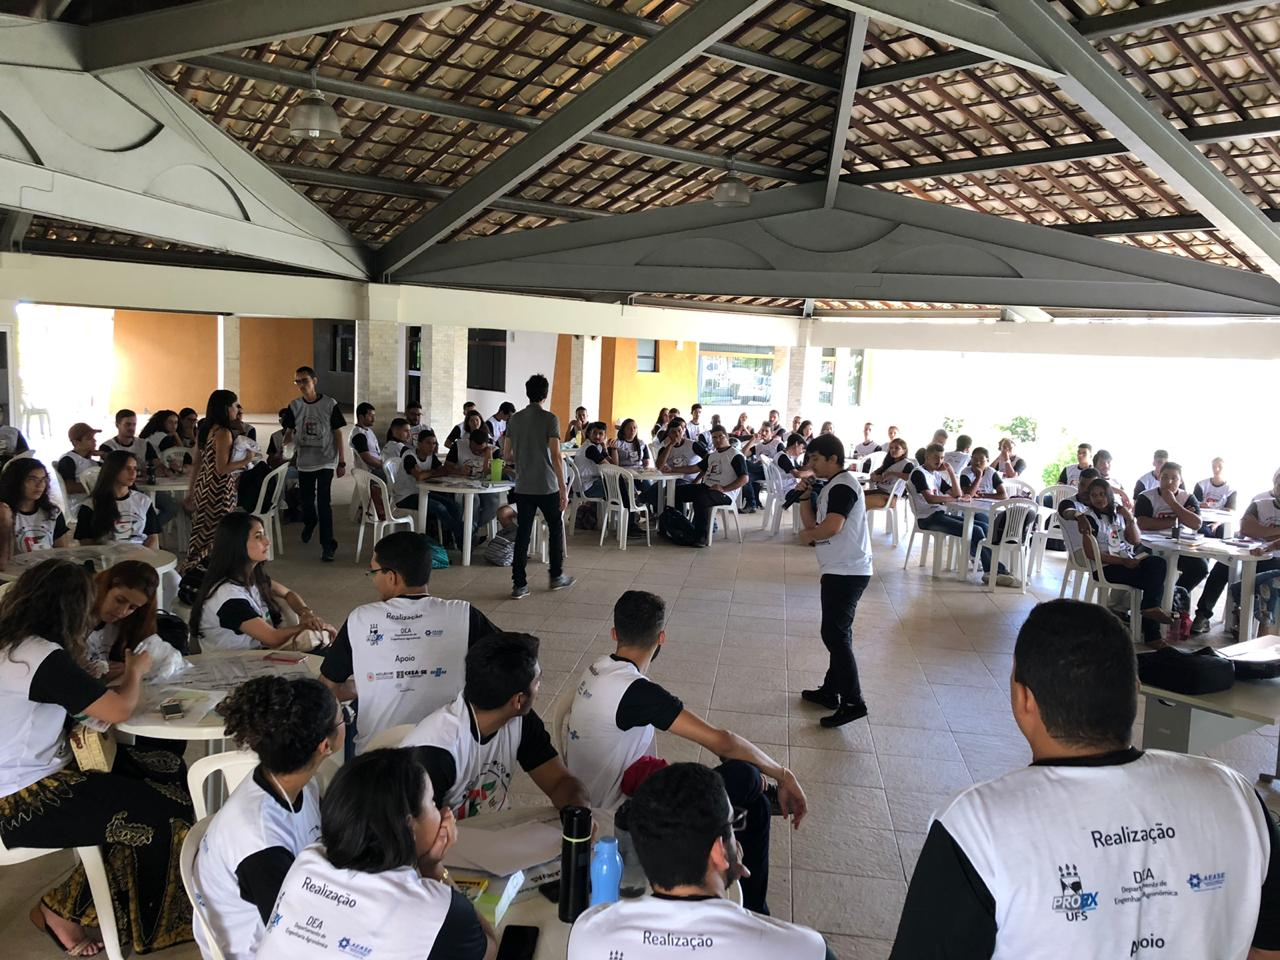
\includegraphics[scale=0.15]{Imagens/primeiro_dia_3.jpg}}
\qquad
\subfigure[ref6][Participantes do programa: 2º dia]{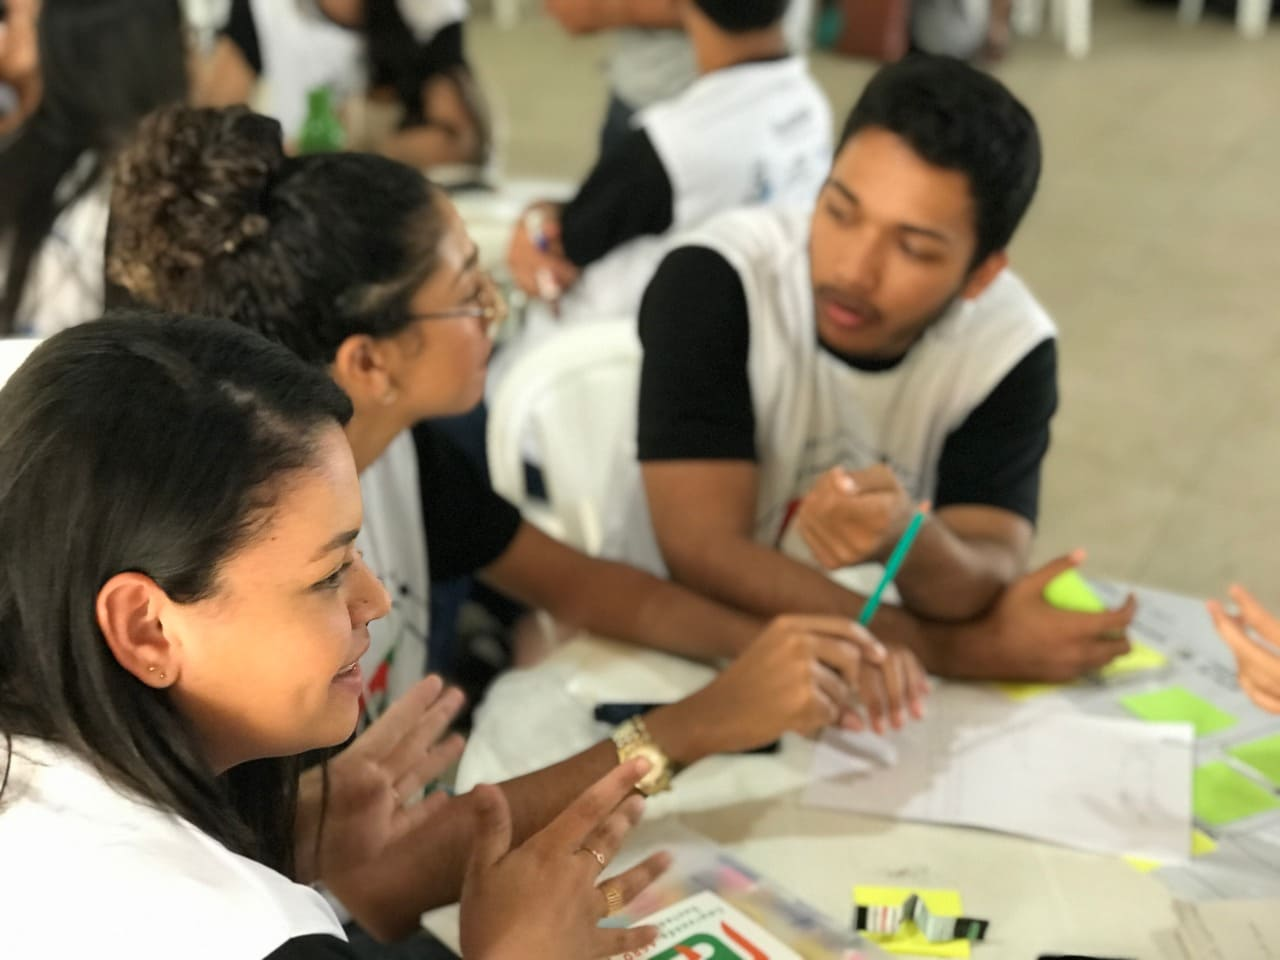
\includegraphics[scale=0.2]{Imagens/primeiro_dia_4.jpg}}
\fonte{O Autor}.
\label{figura_29_1}
\end{figure}


\chapter{2º Workshop Empreenda Agro Sustentável}
\label{app:workshop_2}

\begin{figure}[H]
\FloatBarrier
\center
\caption{\textbf{2º Workshop Empreenda Agro Sustentável}}
\subfigure[ref1][Participantes do programa: 1º dia ]{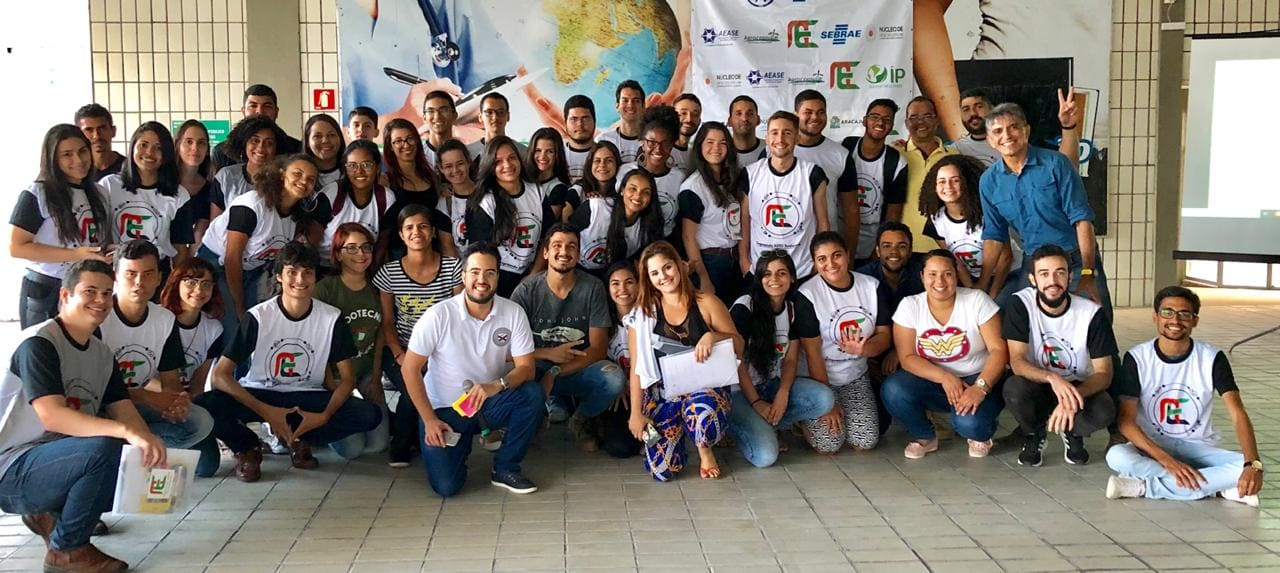
\includegraphics[scale=0.35]{Imagens/segundo_dia_1.jpg}}
\qquad
\subfigure[ref2][Participantes do programa: 2º dia]{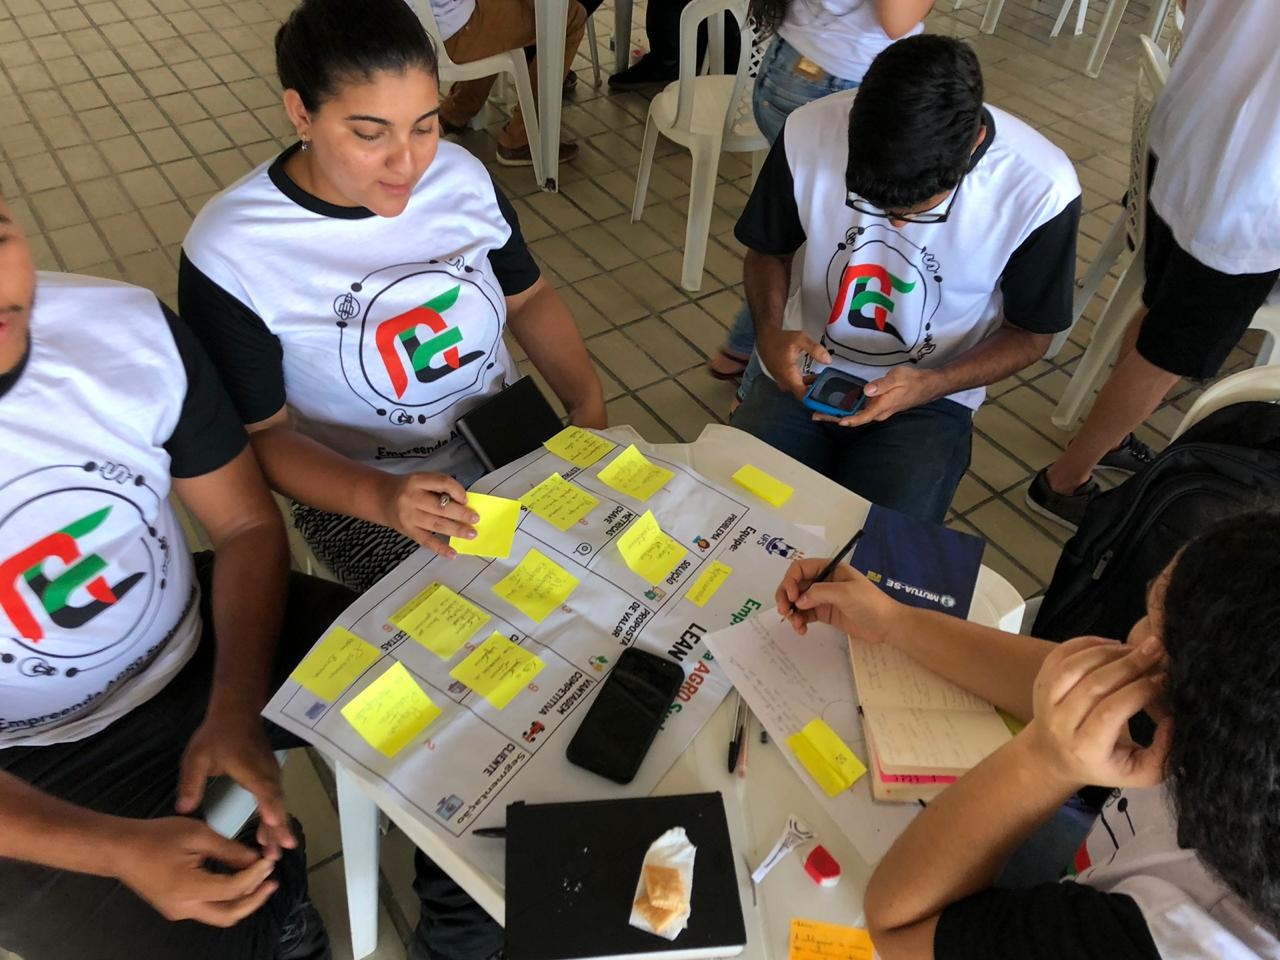
\includegraphics[scale=0.16]{Imagens/segundo_dia_2.jpg}}
\qquad
\subfigure[ref3][Participantes do programa: 2º dia]{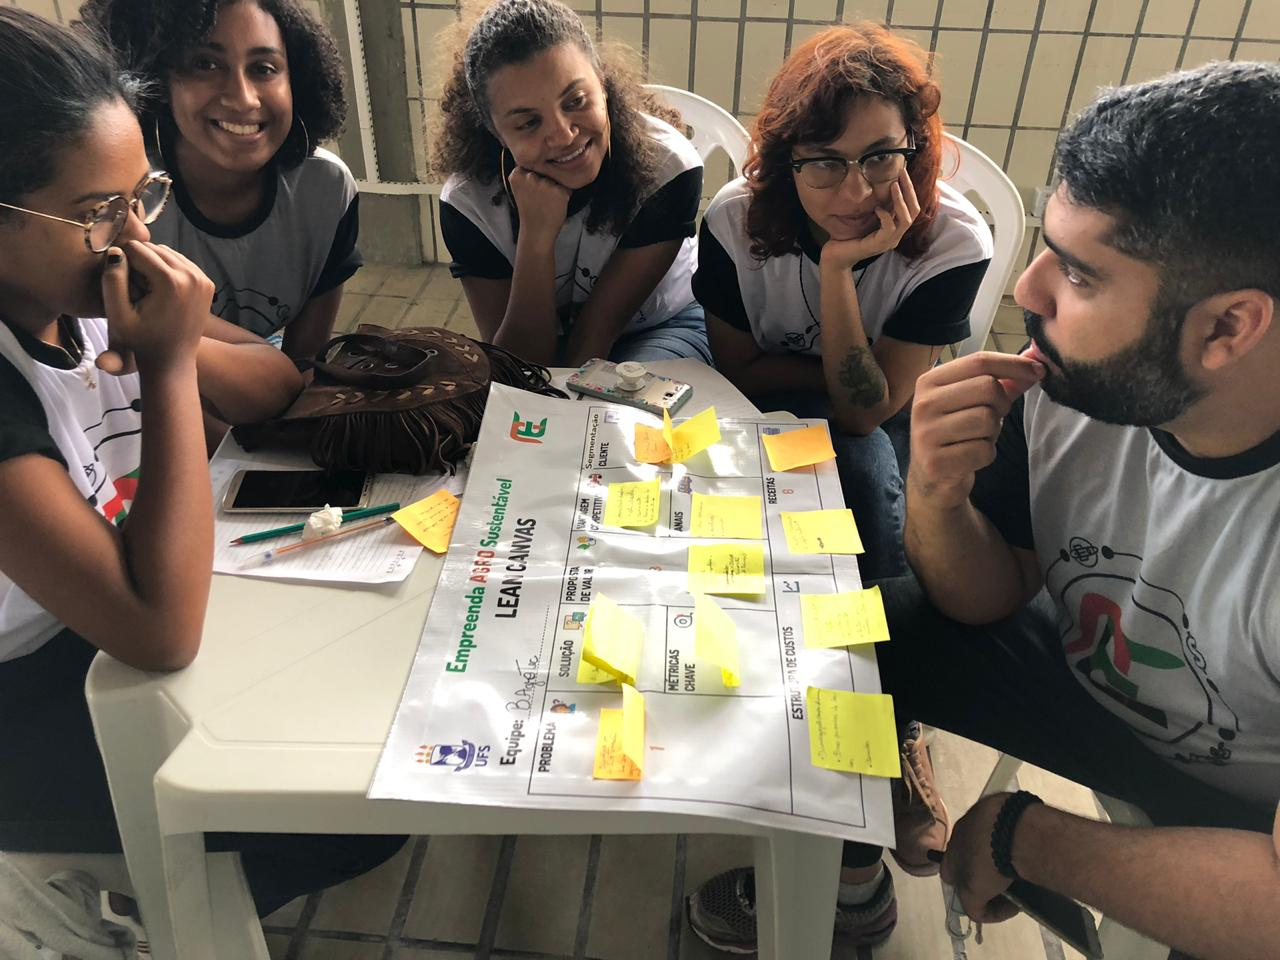
\includegraphics[scale=0.16]{Imagens/segundo_dia_3.jpg}}
\qquad
\subfigure[ref3][Participantes do programa: 2º dia]{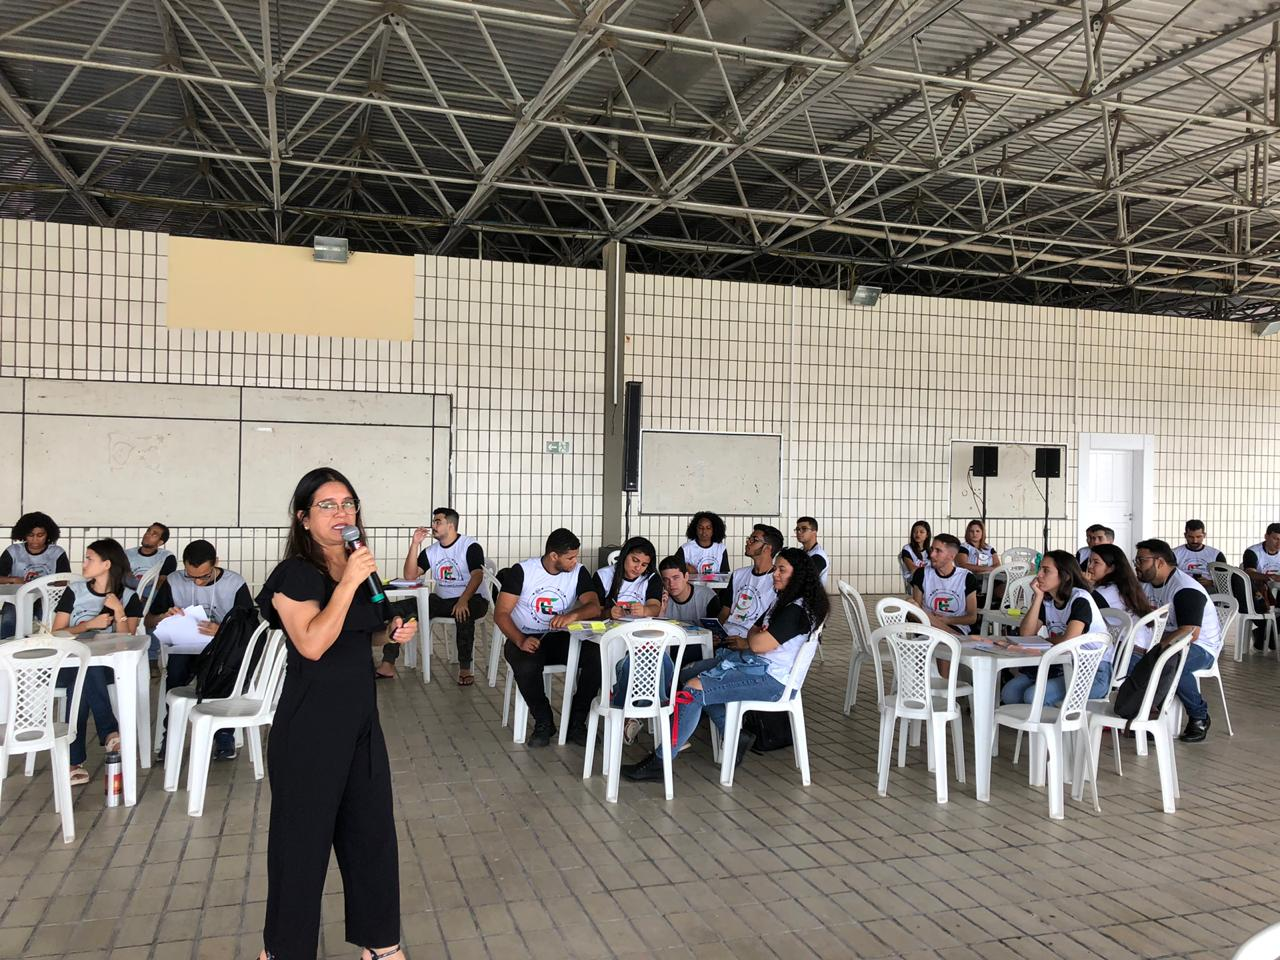
\includegraphics[scale=0.16]{Imagens/segundo_dia_4.jpg}}
\qquad
\subfigure[ref3][Participantes do programa: 2º dia]{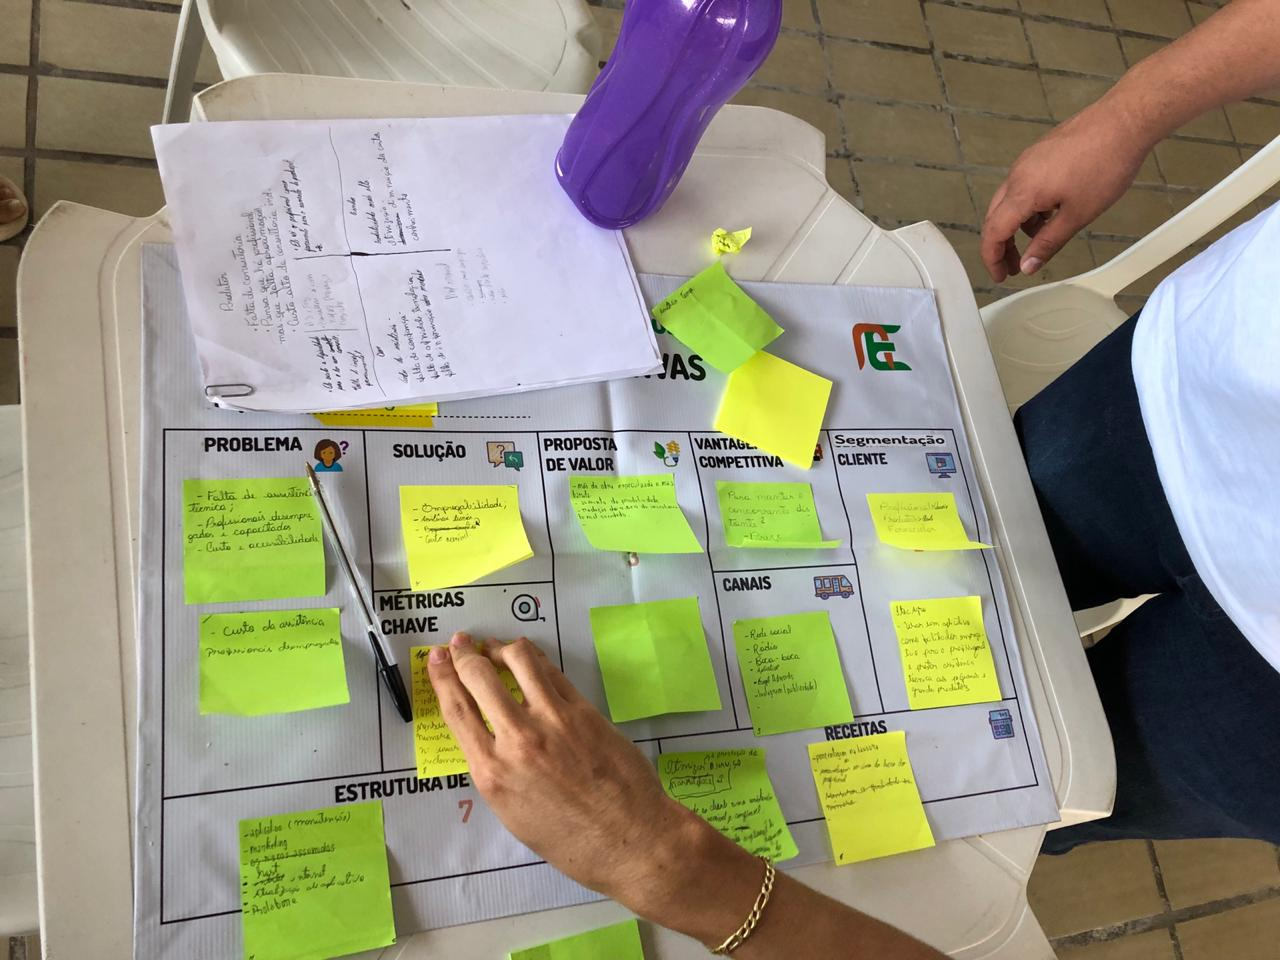
\includegraphics[scale=0.16]{Imagens/segundo_dia_5.jpg}}
\fonte{O Autor}.
\label{figura_segundo_workshop}
\end{figure}

\chapter{3º Workshop: Hackathon Empreenda Agro Sustentável}
\label{app:workshop_hackathon}
\begin{figure}[H]
\FloatBarrier
\center
\caption{\textbf{Hackathon Empreenda Agro Sustentável}}
\subfigure[ref1][Participantes do programa: Hackathon ]{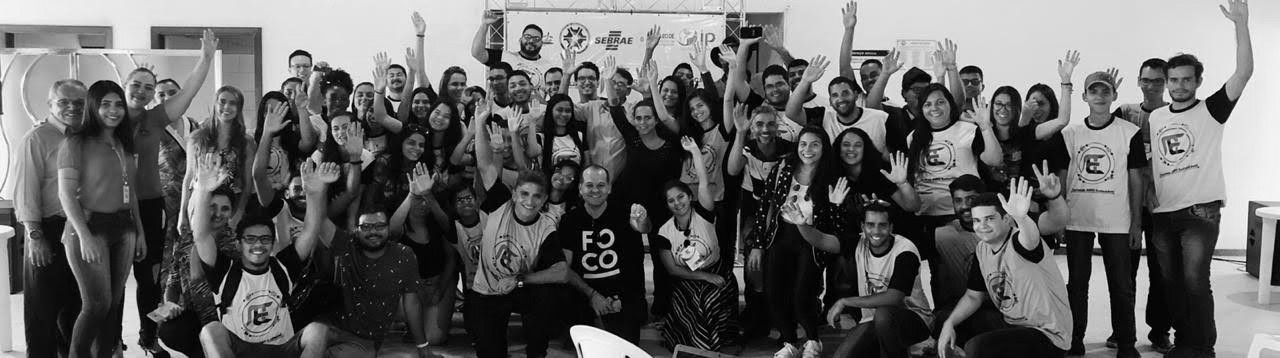
\includegraphics[scale=0.35]{Imagens/terceiro_dia_1.jpg}}
\qquad
\subfigure[ref2][Participantes do programa: Hackathon]{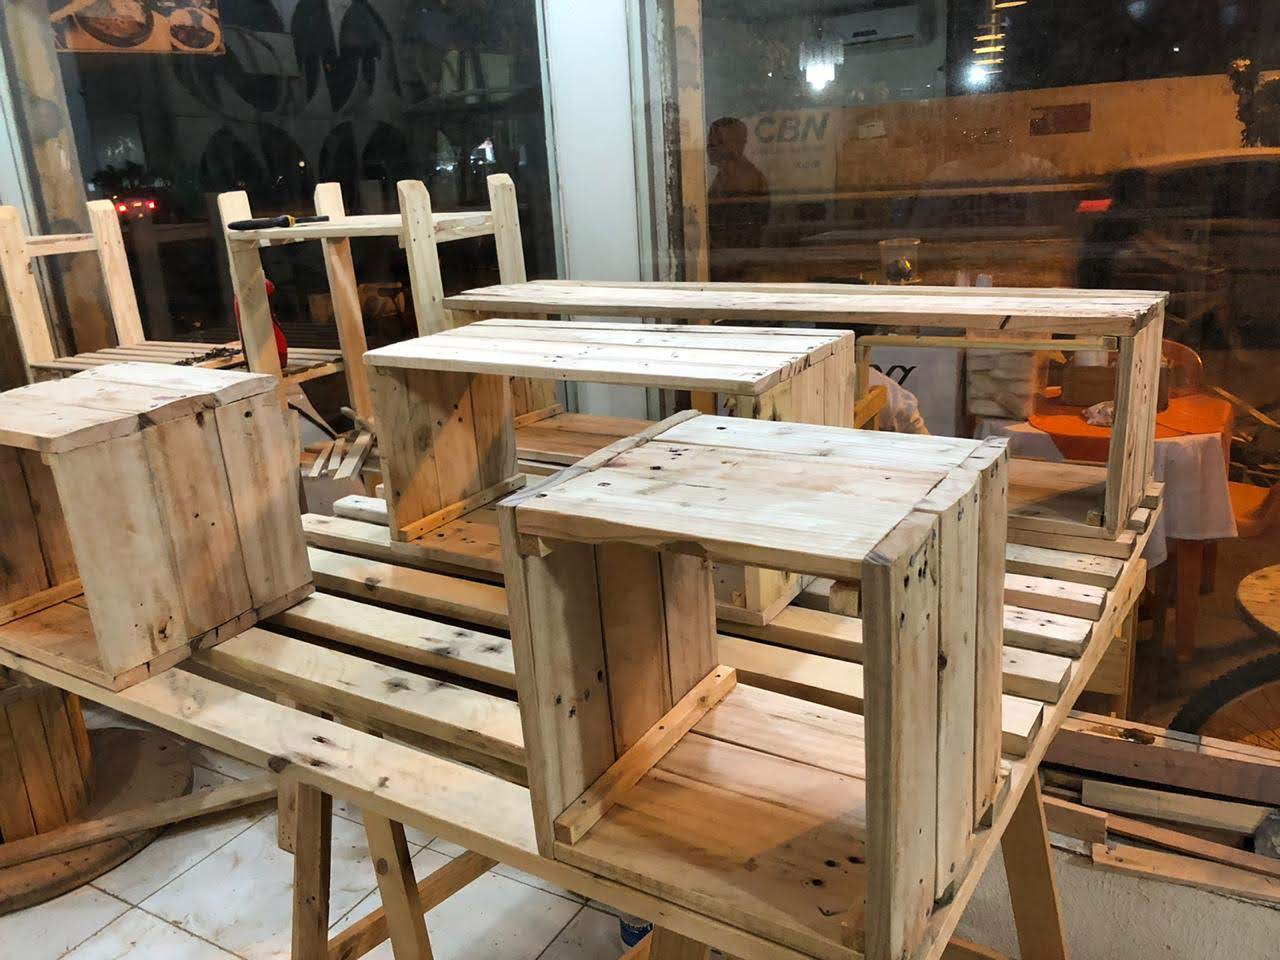
\includegraphics[scale=0.15]{Imagens/terceiro_dia_2.jpg}}
\qquad
\subfigure[ref3][Participantes do programa: Hackathon]{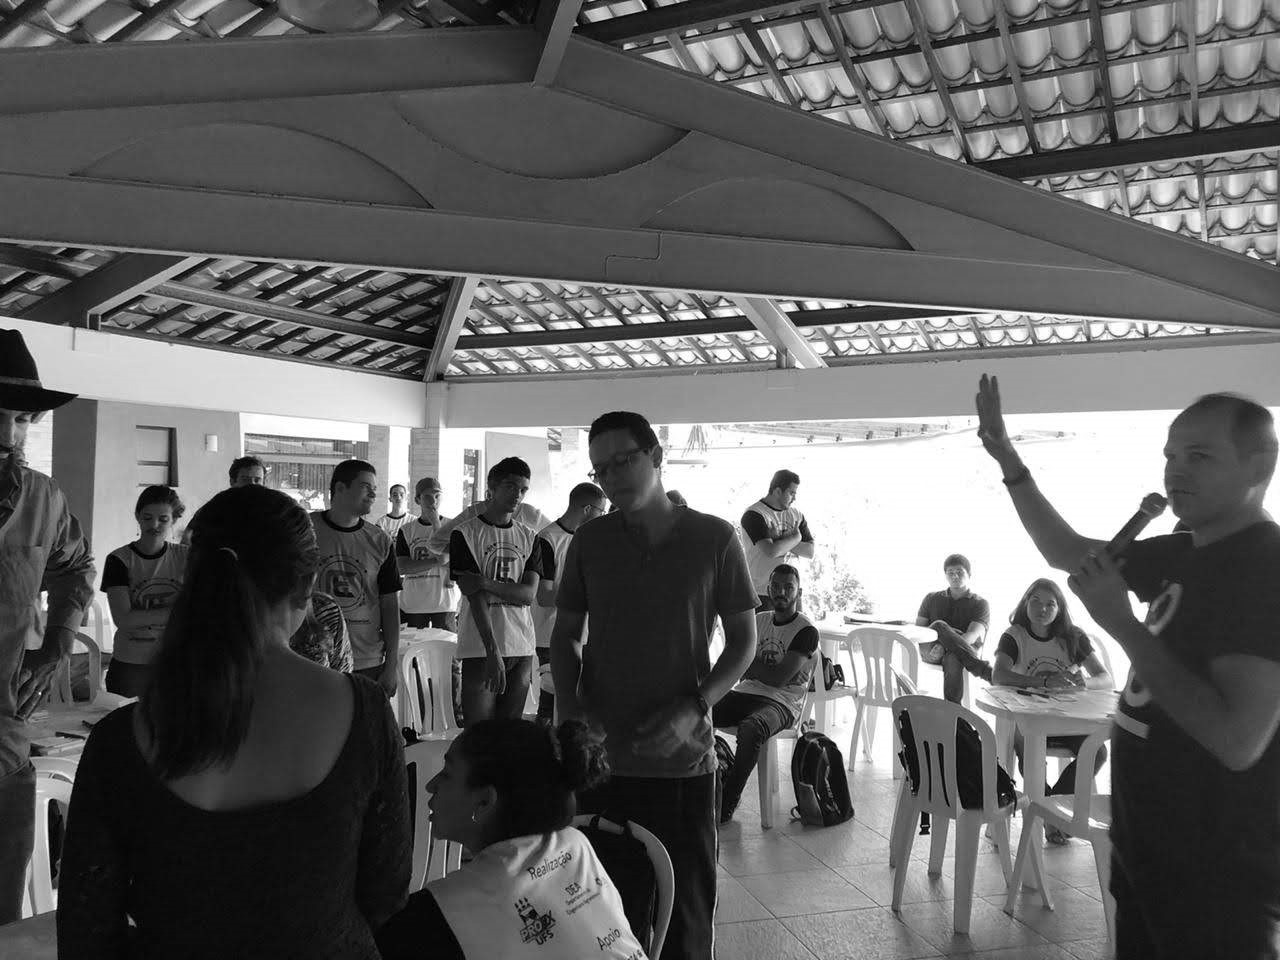
\includegraphics[scale=0.15]{Imagens/terceiro_dia_3.jpg}}
\subfigure[ref4][Protótipos: Hackathon]{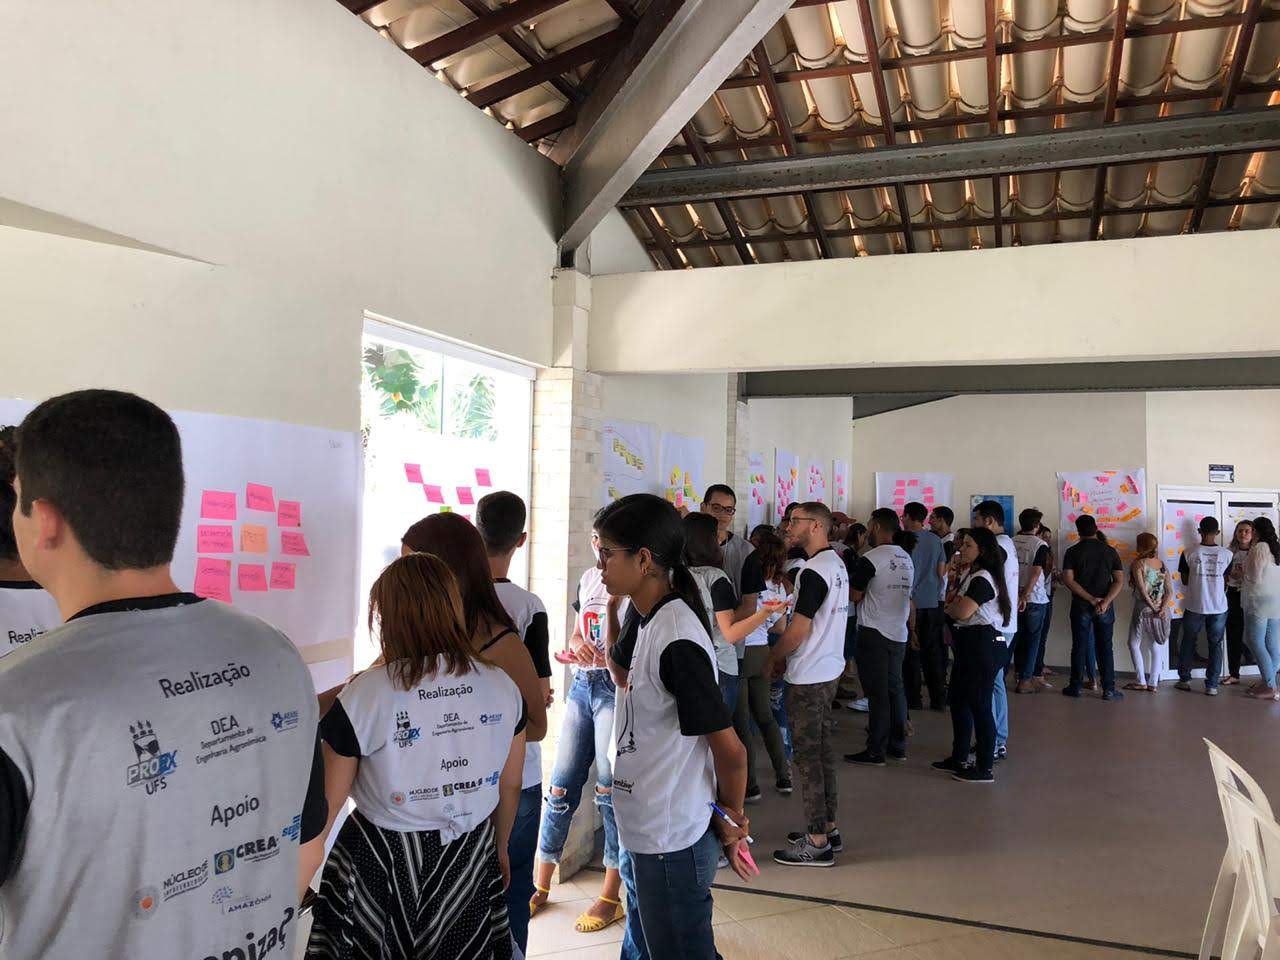
\includegraphics[scale=0.08]{Imagens/terceiro_dia_4.jpg}}
\qquad
\subfigure[ref5][Protótipos: Hackathon]{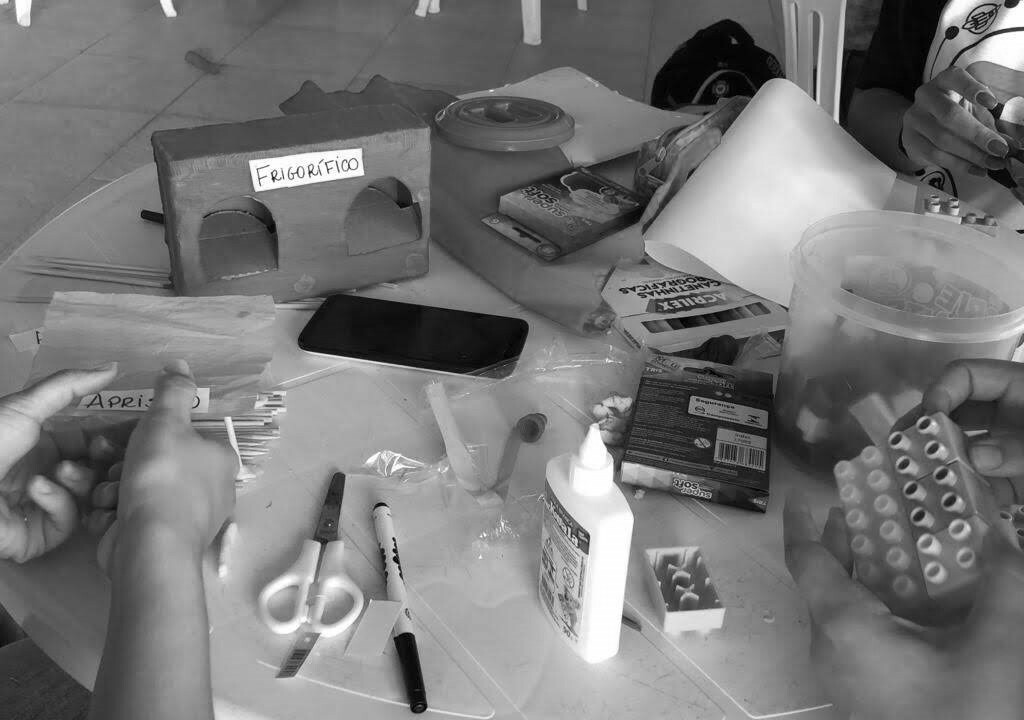
\includegraphics[scale=0.15]{Imagens/terceiro_dia_5.jpg}}
\fonte{O Autor}.
\label{figura_51}
\end{figure}


\chapter{4º Workshop: Demoday}
\label{app:workshop_demoday}

\begin{figure}[H]
\center
\FloatBarrier
\caption{\textbf{Demoday Empreenda Agro Sustentável}}
\subfigure[ref1][Evento  Demoday]{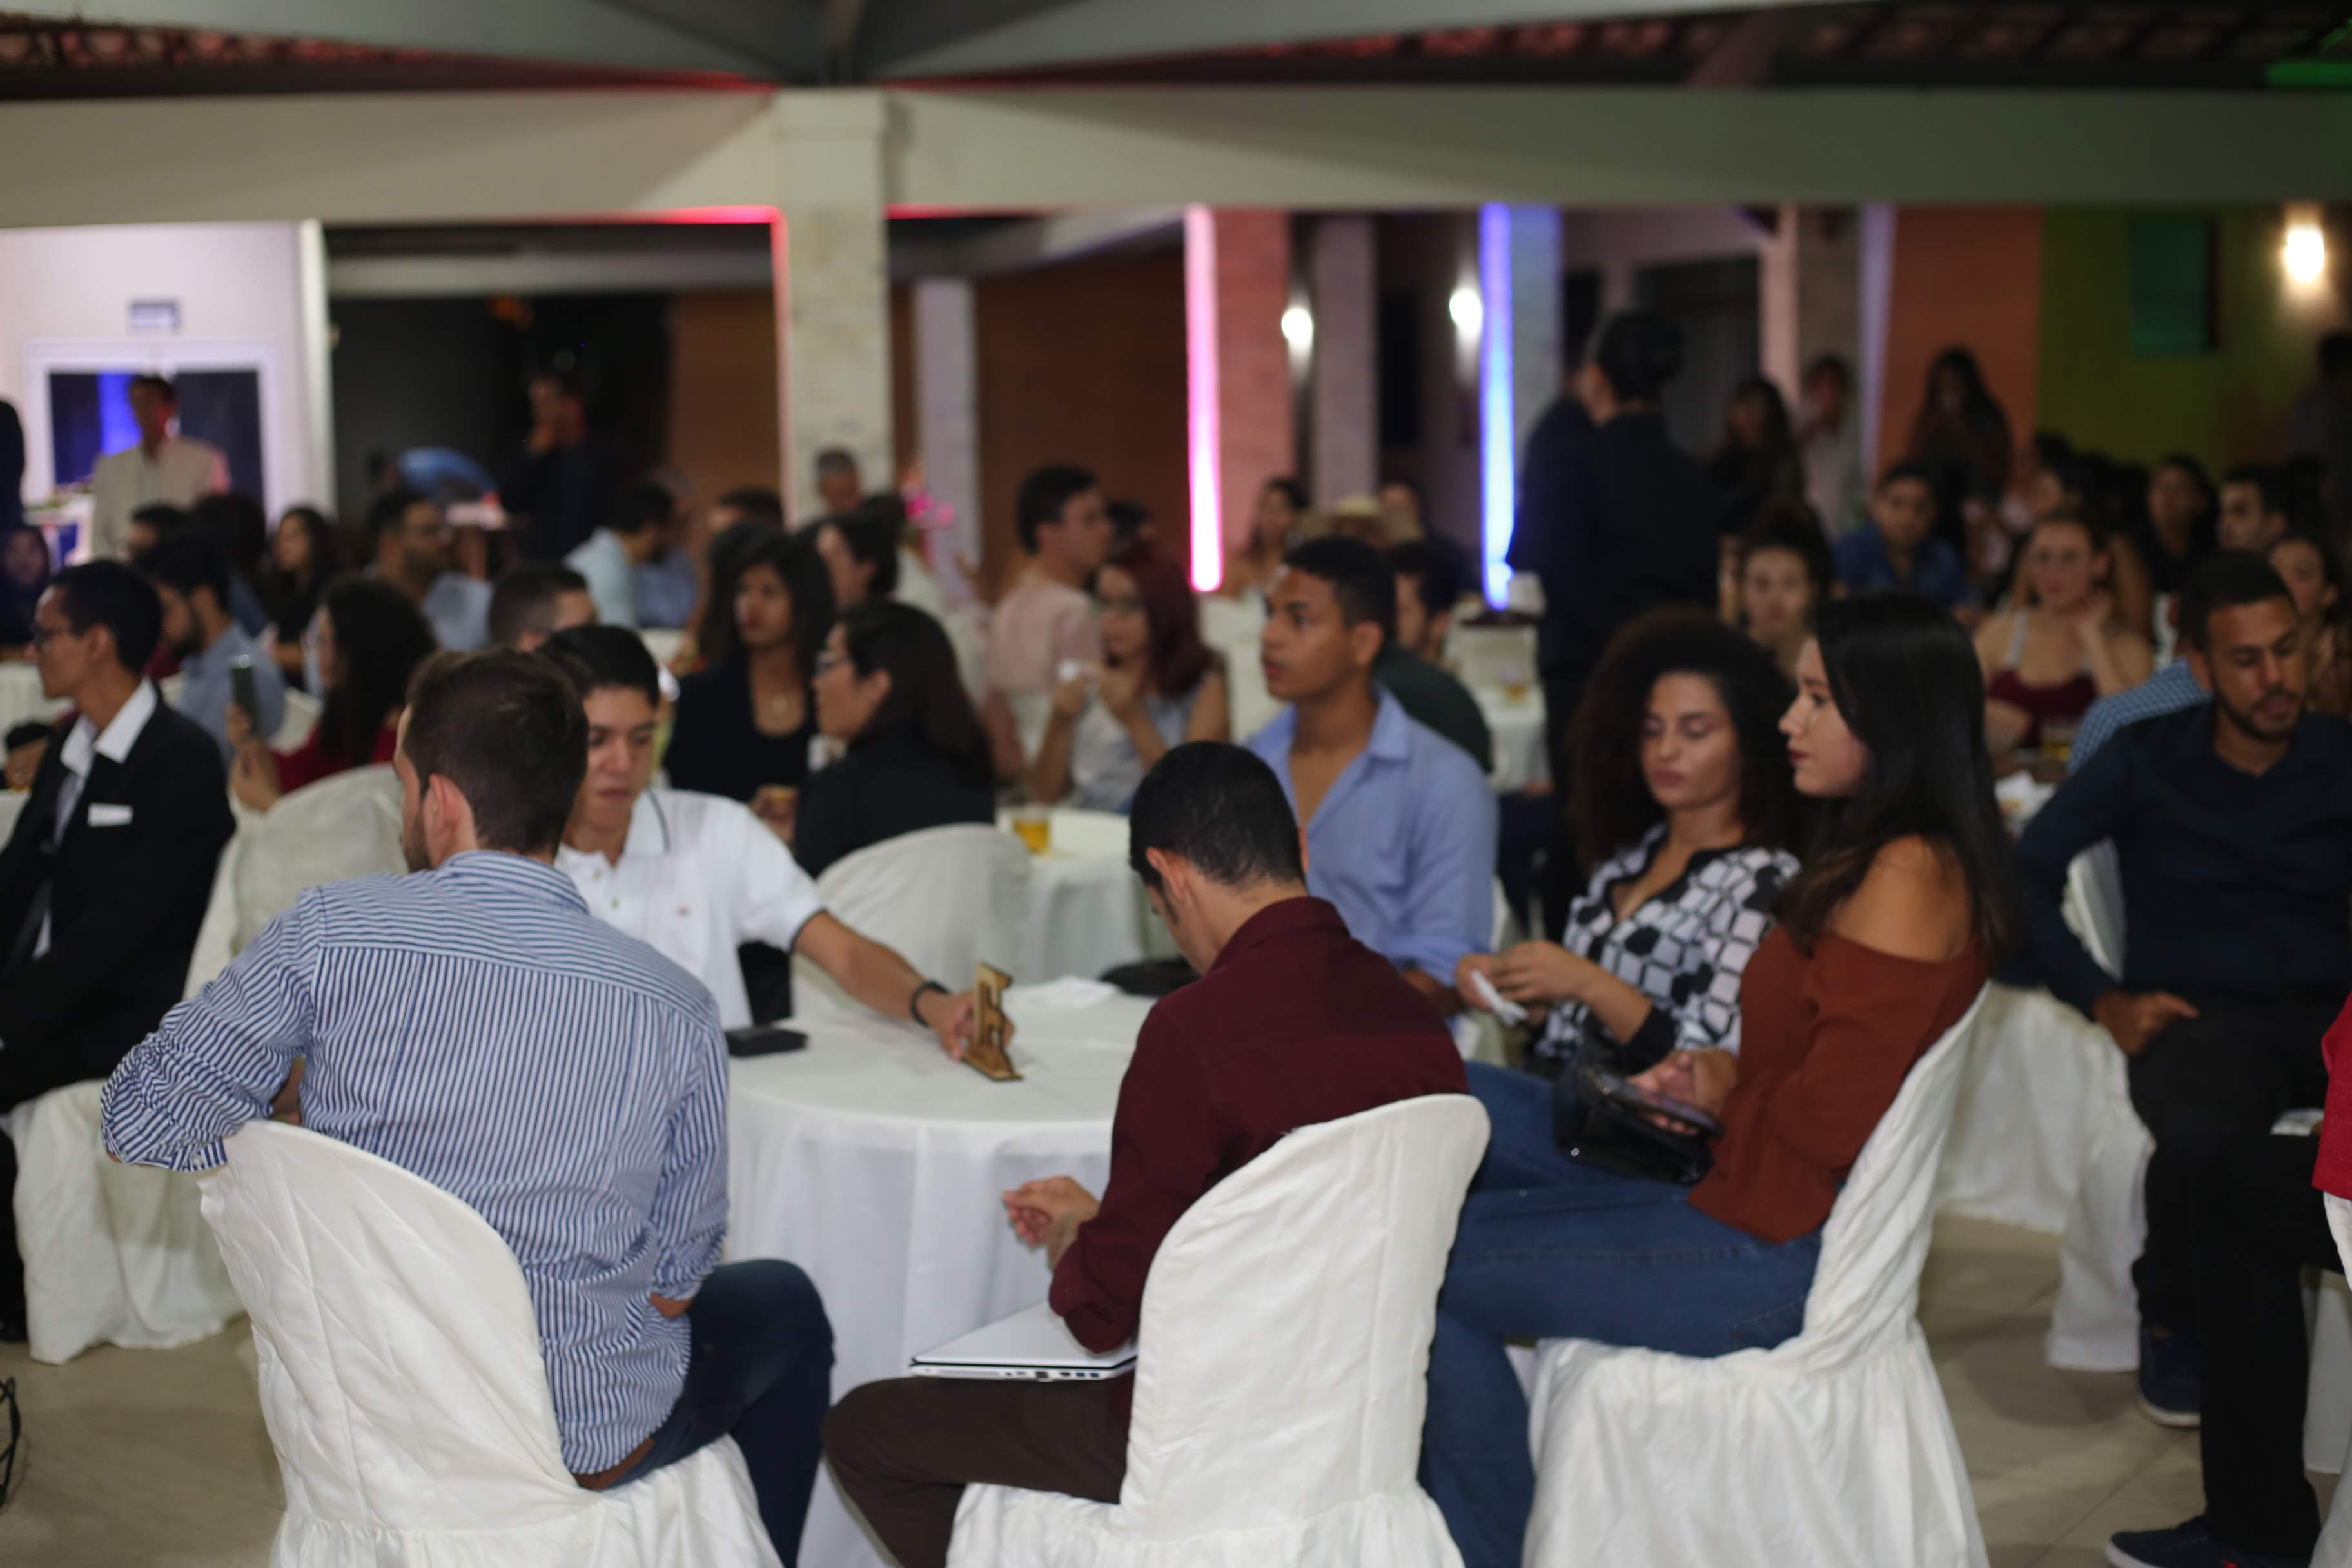
\includegraphics[scale=0.05]{Imagens/demoday_3.jpg}}
\qquad
\subfigure[ref2][Premiação simbólica]{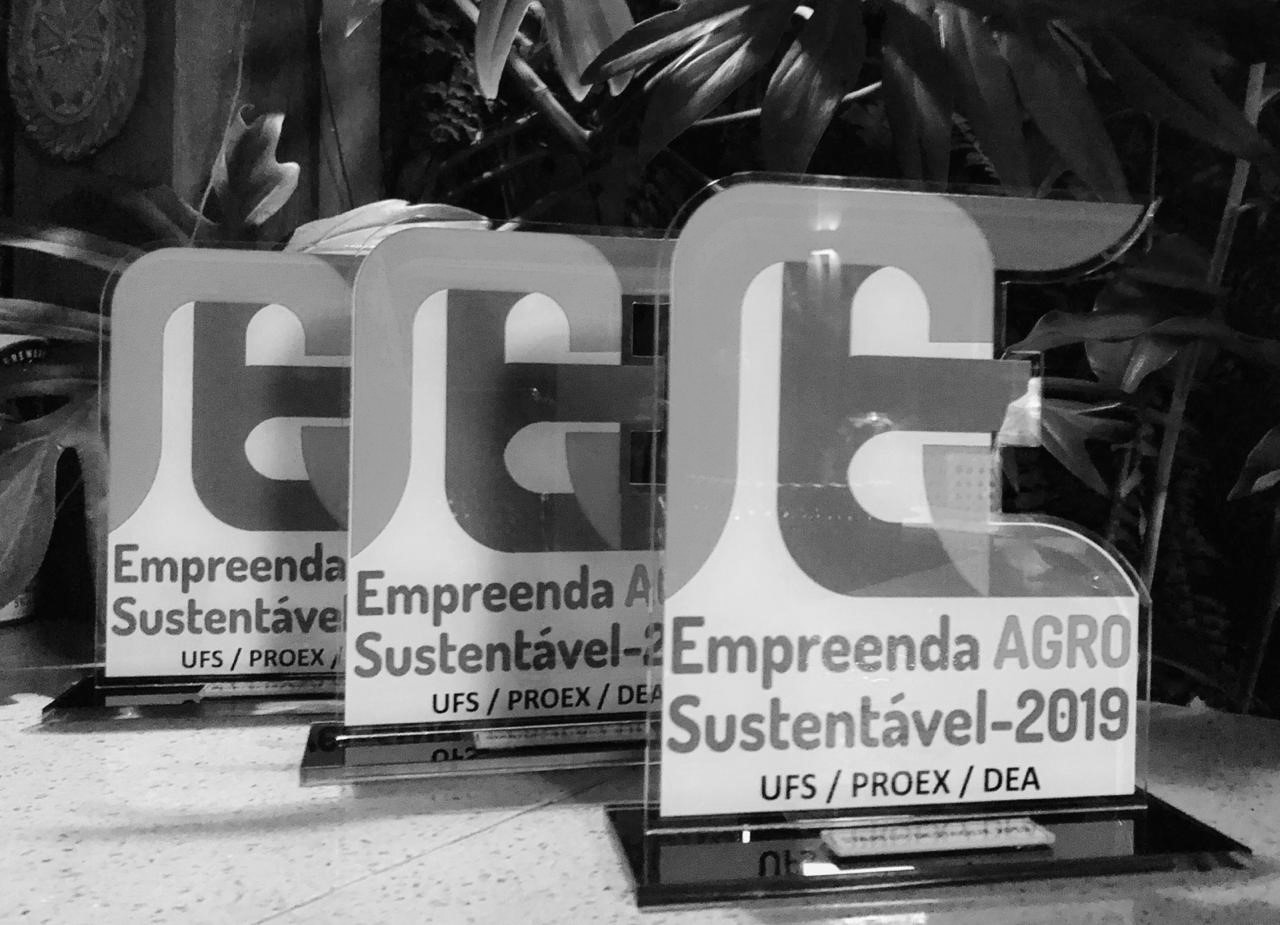
\includegraphics[scale=0.05]{Imagens/demoday_premiacao.jpg}}
\qquad
\subfigure[ref3][Apresentação das propostas: Tecno Coco]{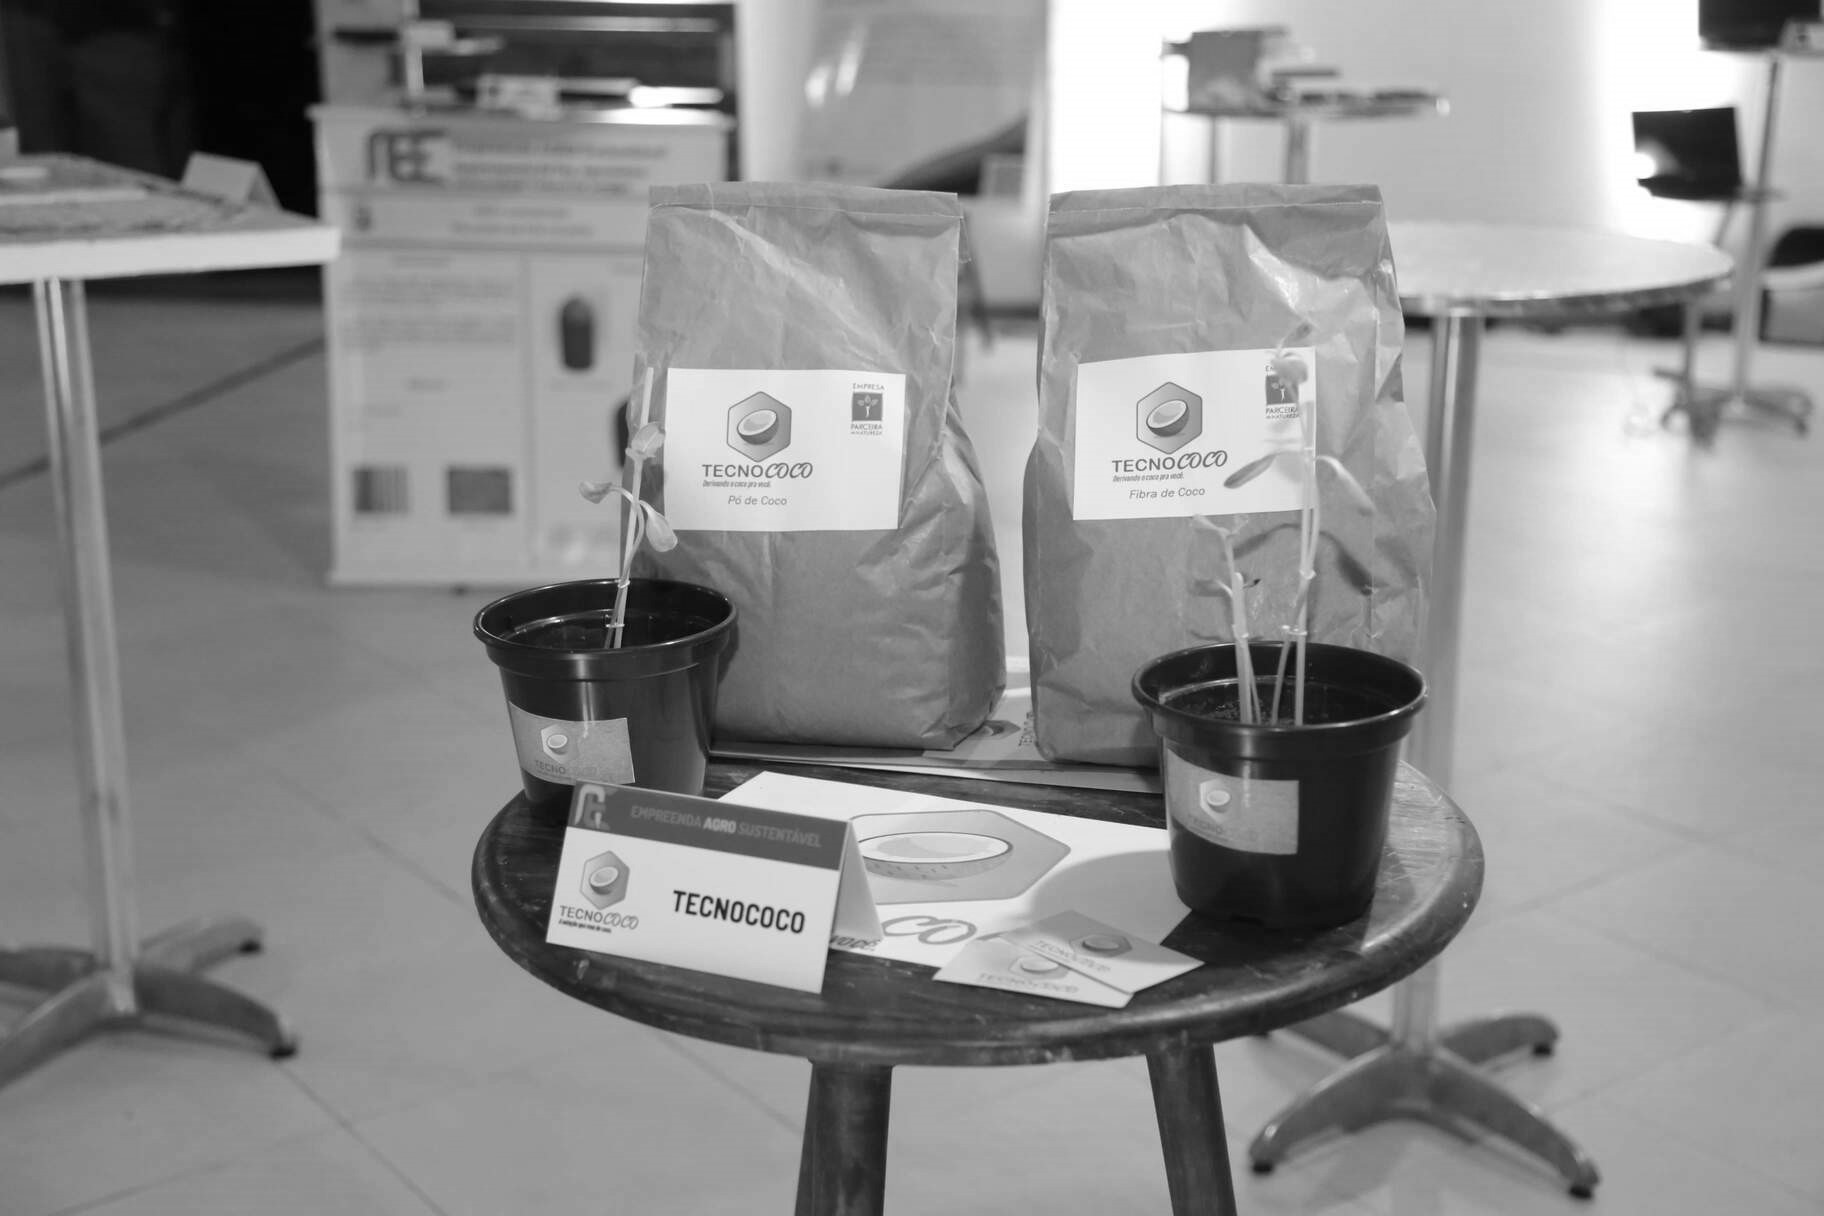
\includegraphics[scale=0.05]{Imagens/demoday_15.jpg}}
\qquad
\subfigure[ref4][Protótipos desenvolvidos: MAMP]{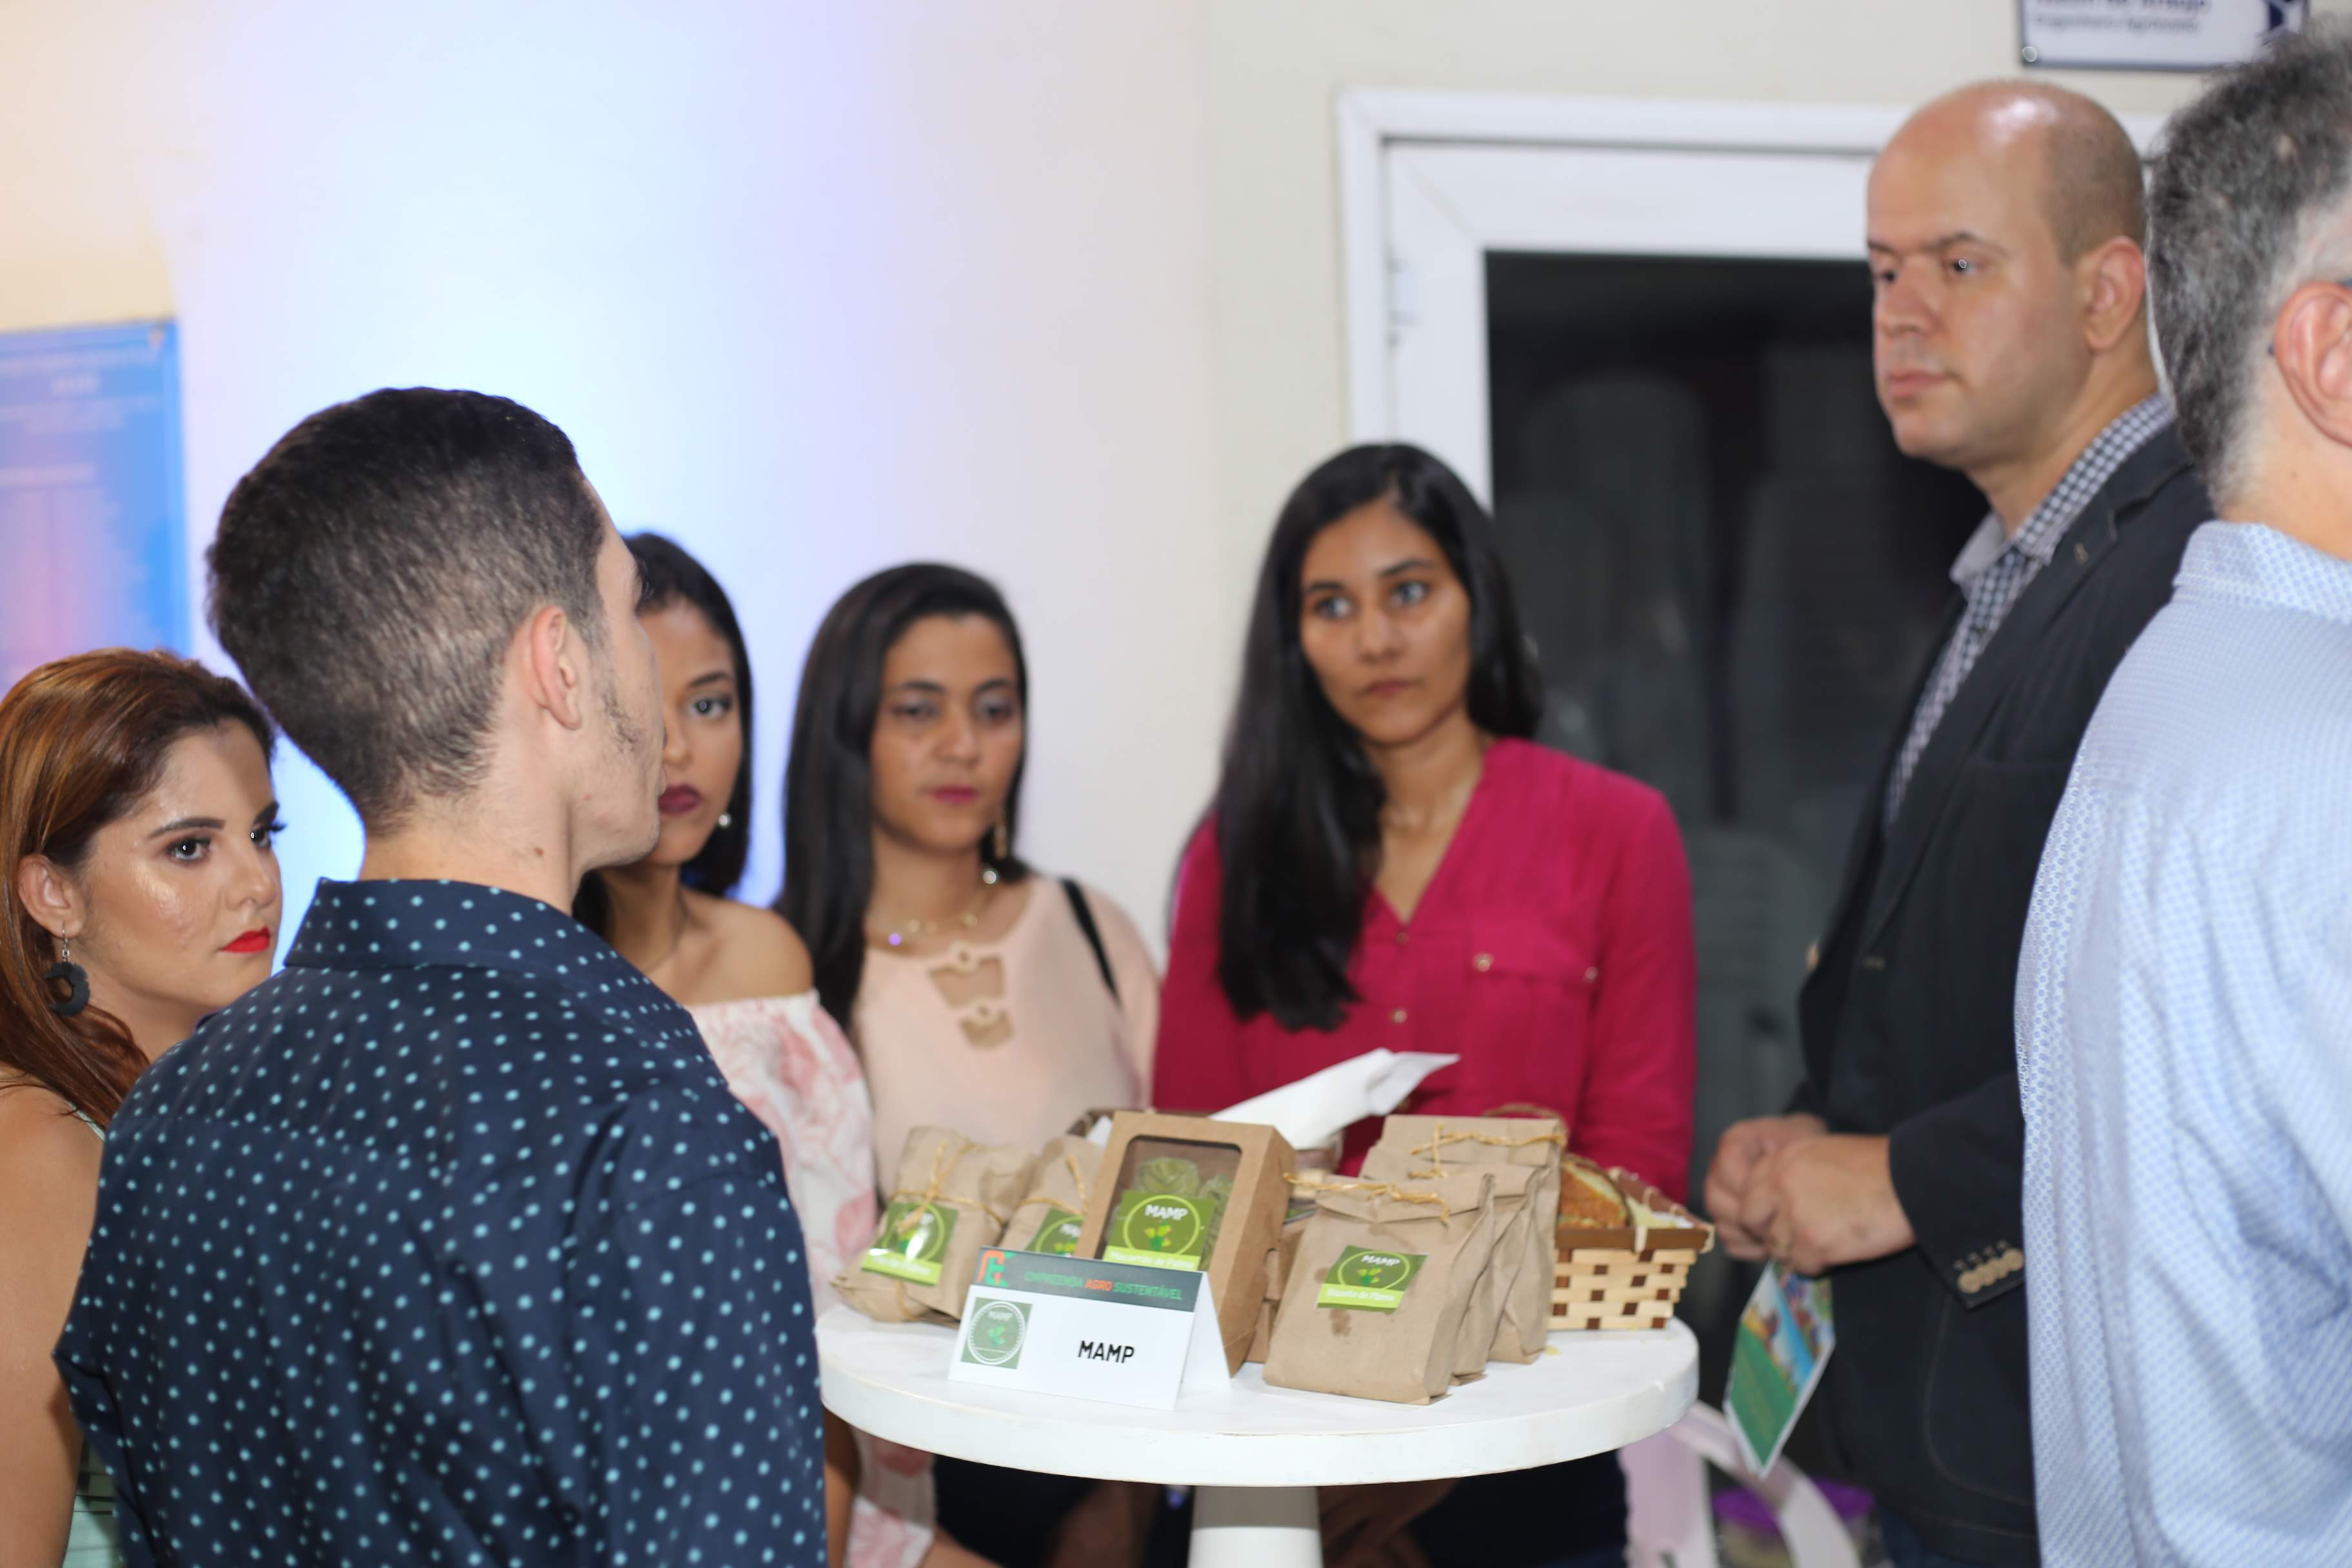
\includegraphics[scale=0.05]{Imagens/demoday_12.jpg}}
\qquad
\subfigure[ref5][Convidados: Ranagro]{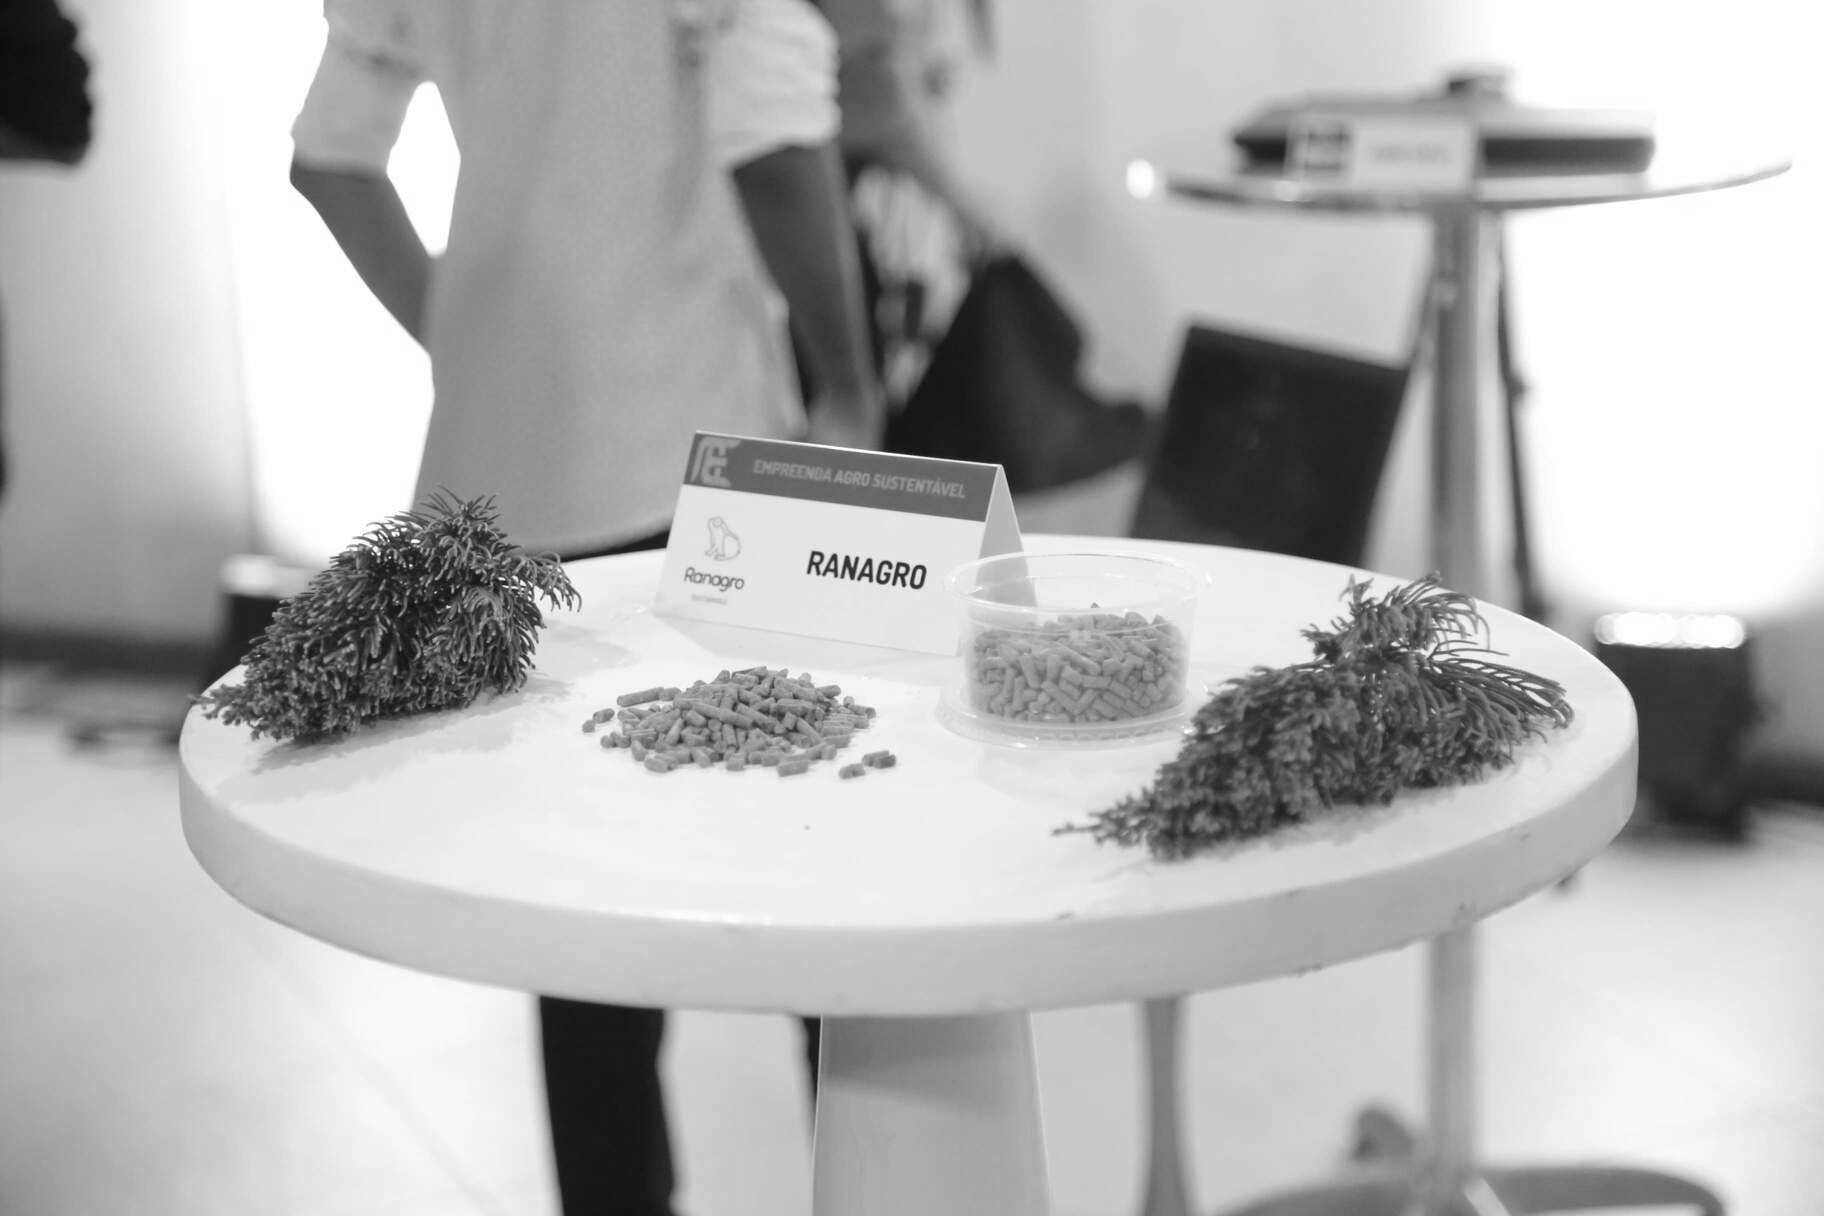
\includegraphics[scale=0.05]{Imagens/demoday_10.jpg}}
\qquad
\subfigure[ref6][Apresentação das propostas: La Flora Pet]{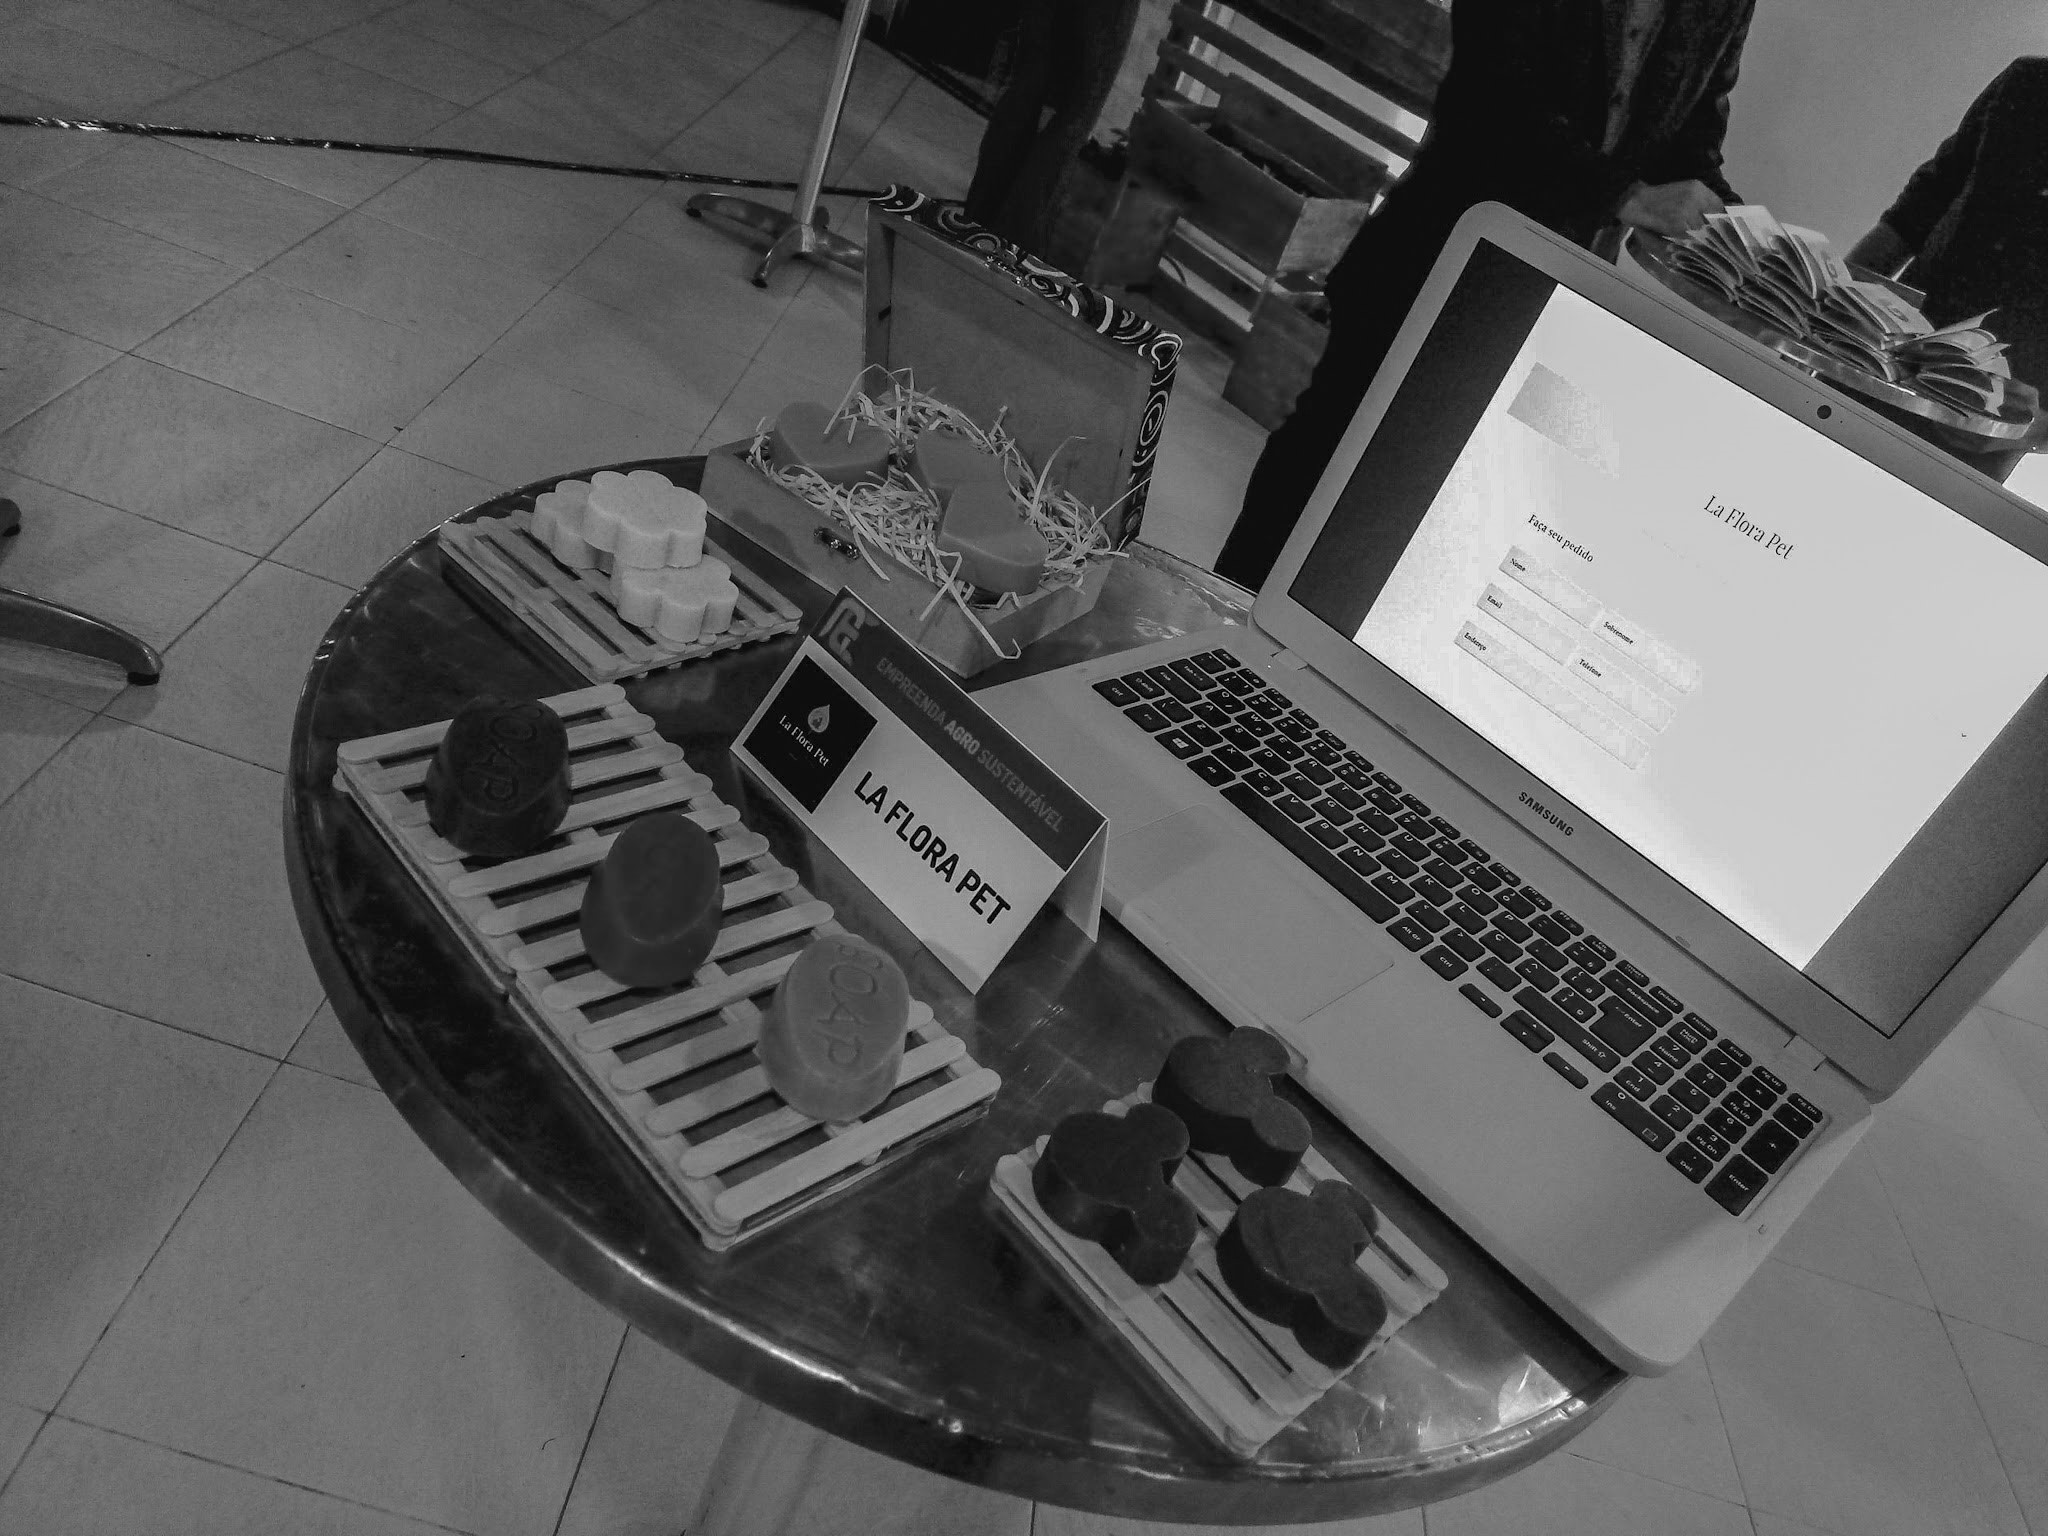
\includegraphics[scale=0.05]{Imagens/demoday_6.jpg}}
\fonte{O Autor}.
\label{figura_35}
\end{figure}

\begin{figure}[H]
\center
\FloatBarrier
\caption{\textbf{Exemplos de "Minimum Commercially Viable Product" (MCVP) desenvolvidos durante o programa}}
\subfigure[ref1][MCVP desenvolvido por Tecnococo]{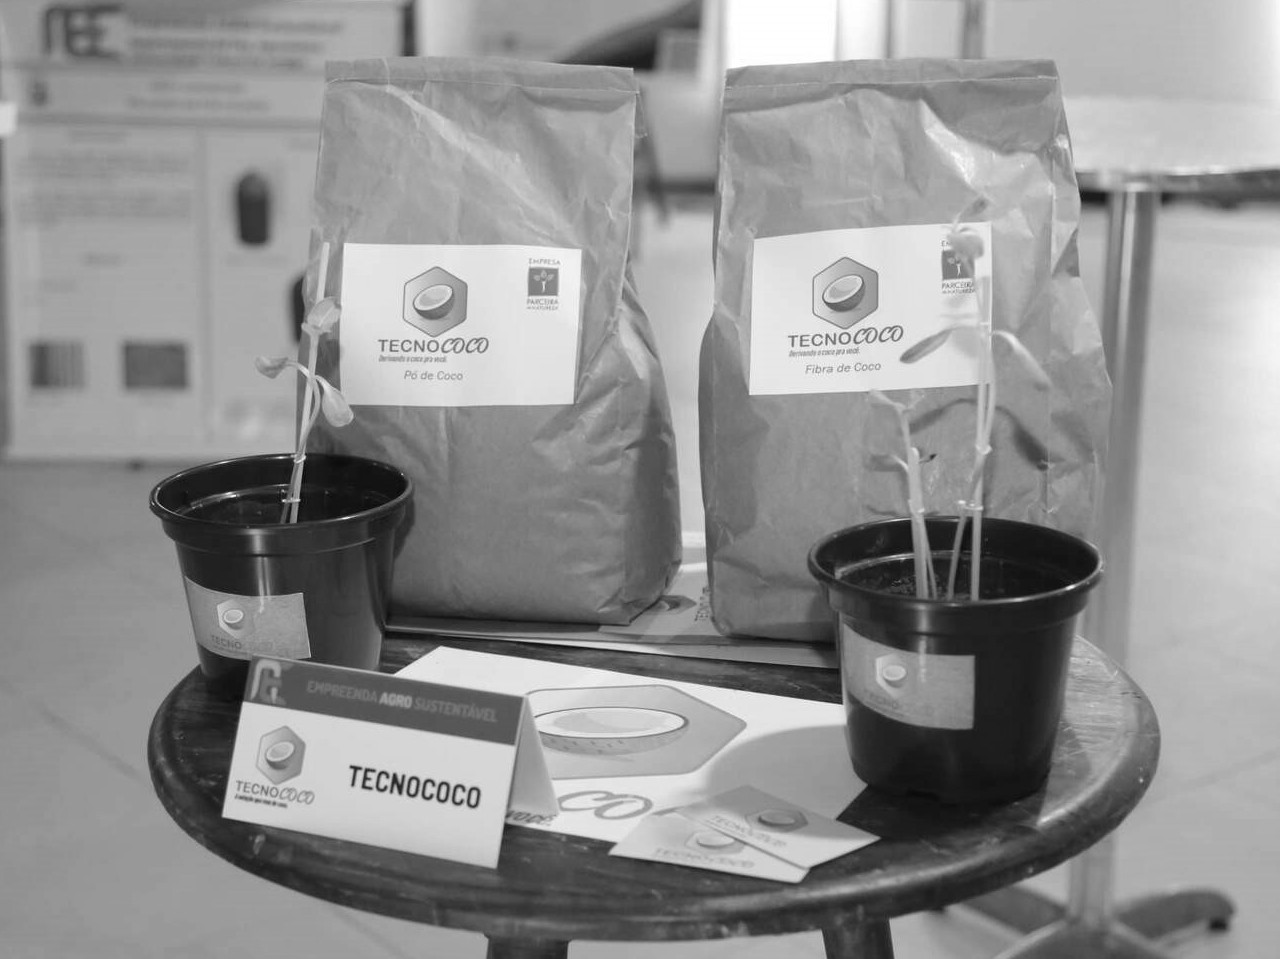
\includegraphics[scale=0.05]{Imagens/prototipo_1.jpg}}
\qquad
\subfigure[ref4][MCVP desenvolvido po La Flora Pet]{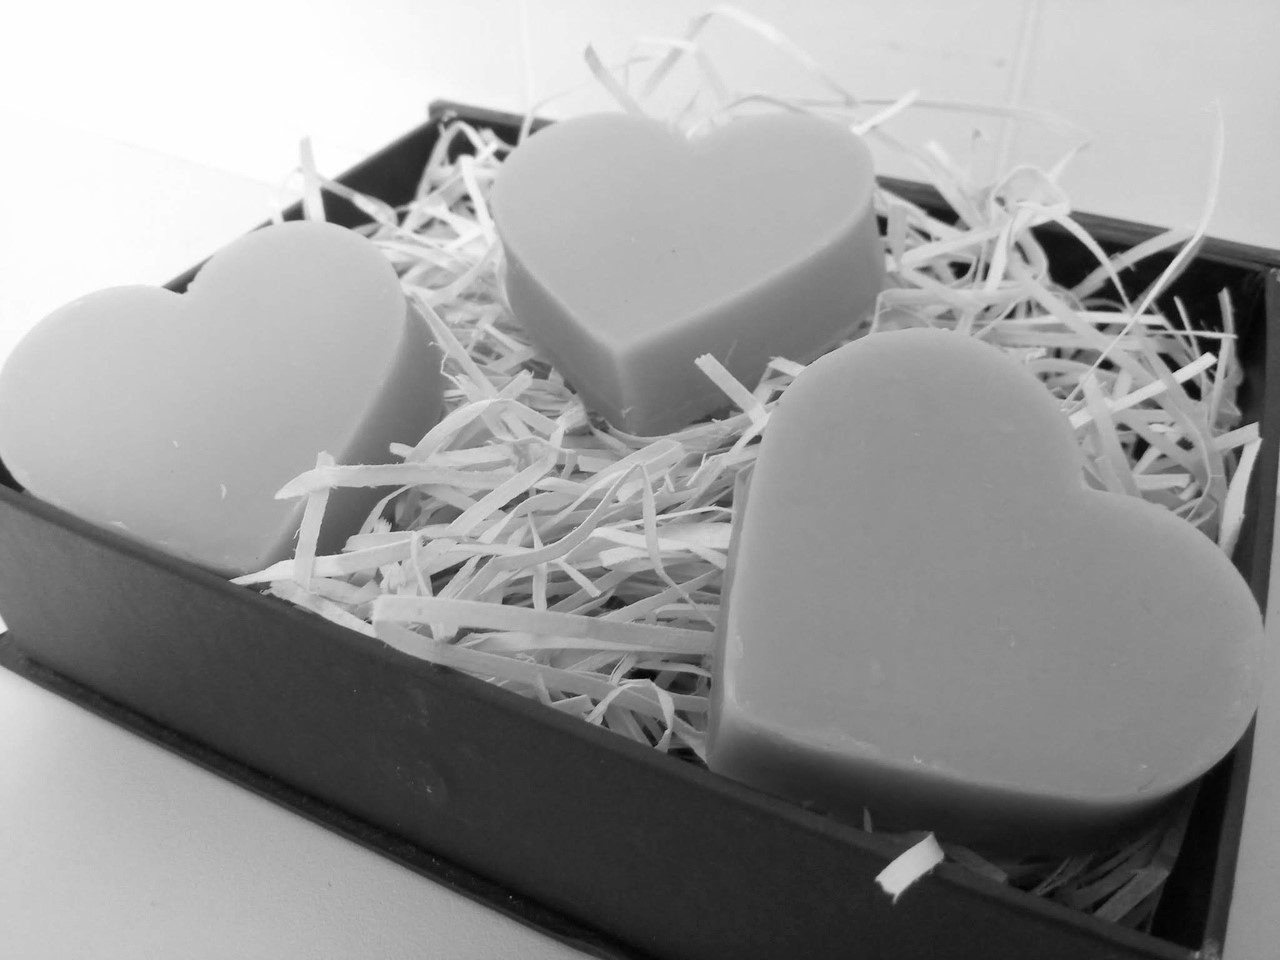
\includegraphics[scale=0.05]{Imagens/prototipo_4.jpg}}
\qquad
\subfigure[ref2][MCVP desenvolvido  MAMP]{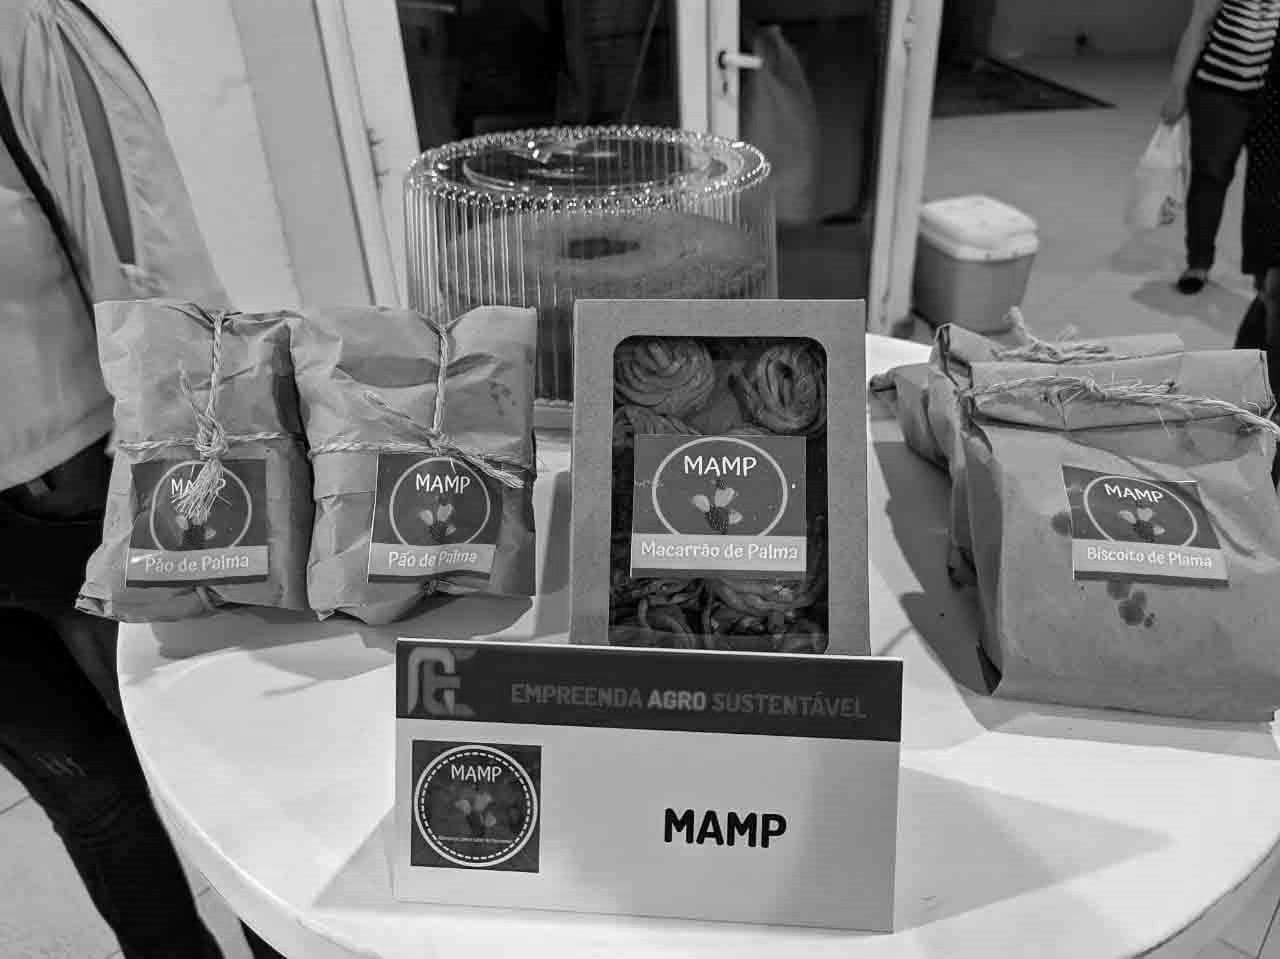
\includegraphics[scale=0.14]{Imagens/prototipo_2.jpg}}
\qquad
\subfigure[ref3][MCVP desenvolvido por Horta House ]{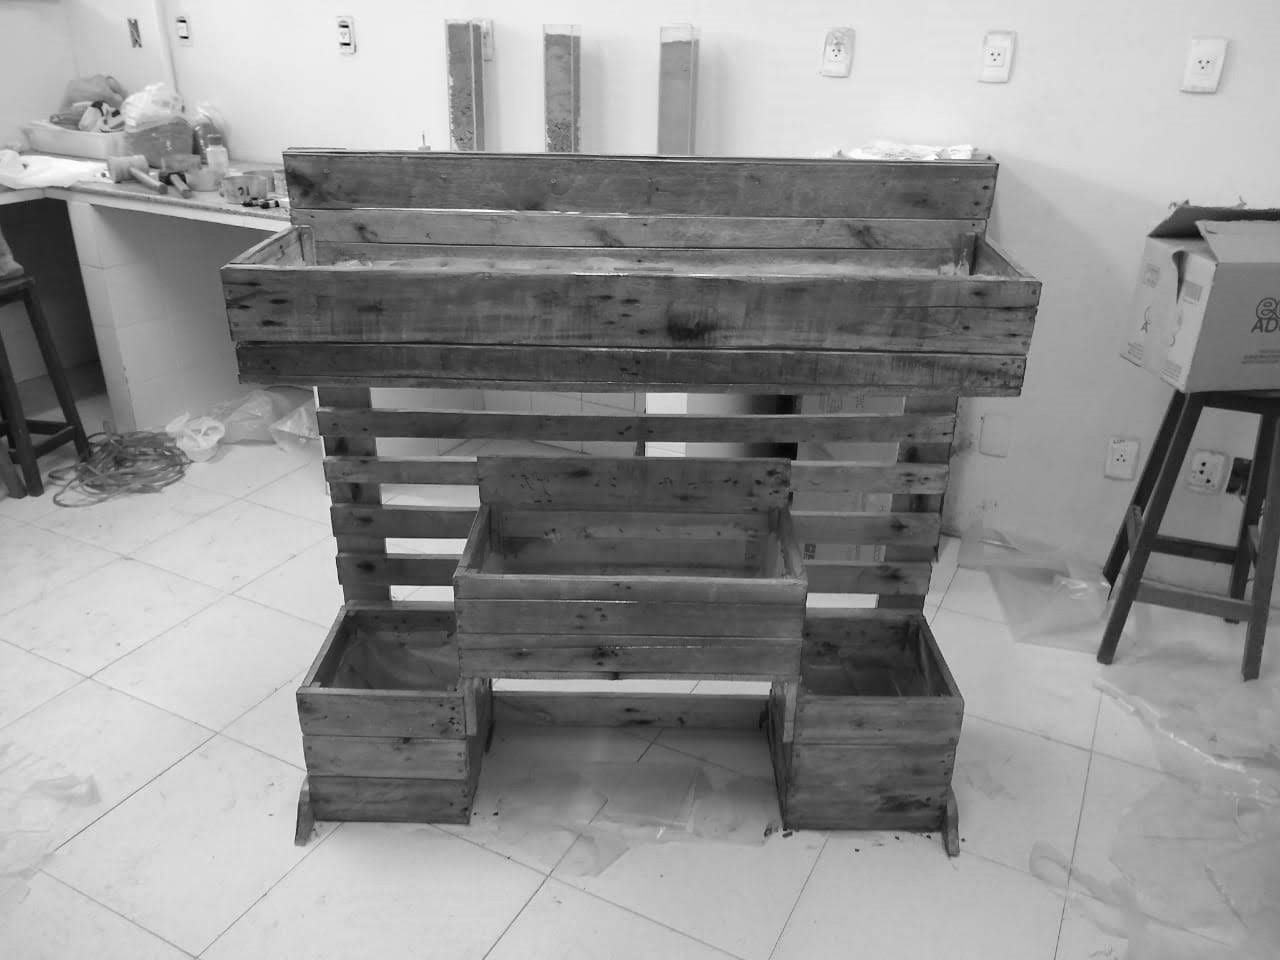
\includegraphics[scale=0.14]{Imagens/prototipo_3.jpg}}
\qquad
\subfigure[ref2][MCVP desenvolvido por Itecagro]{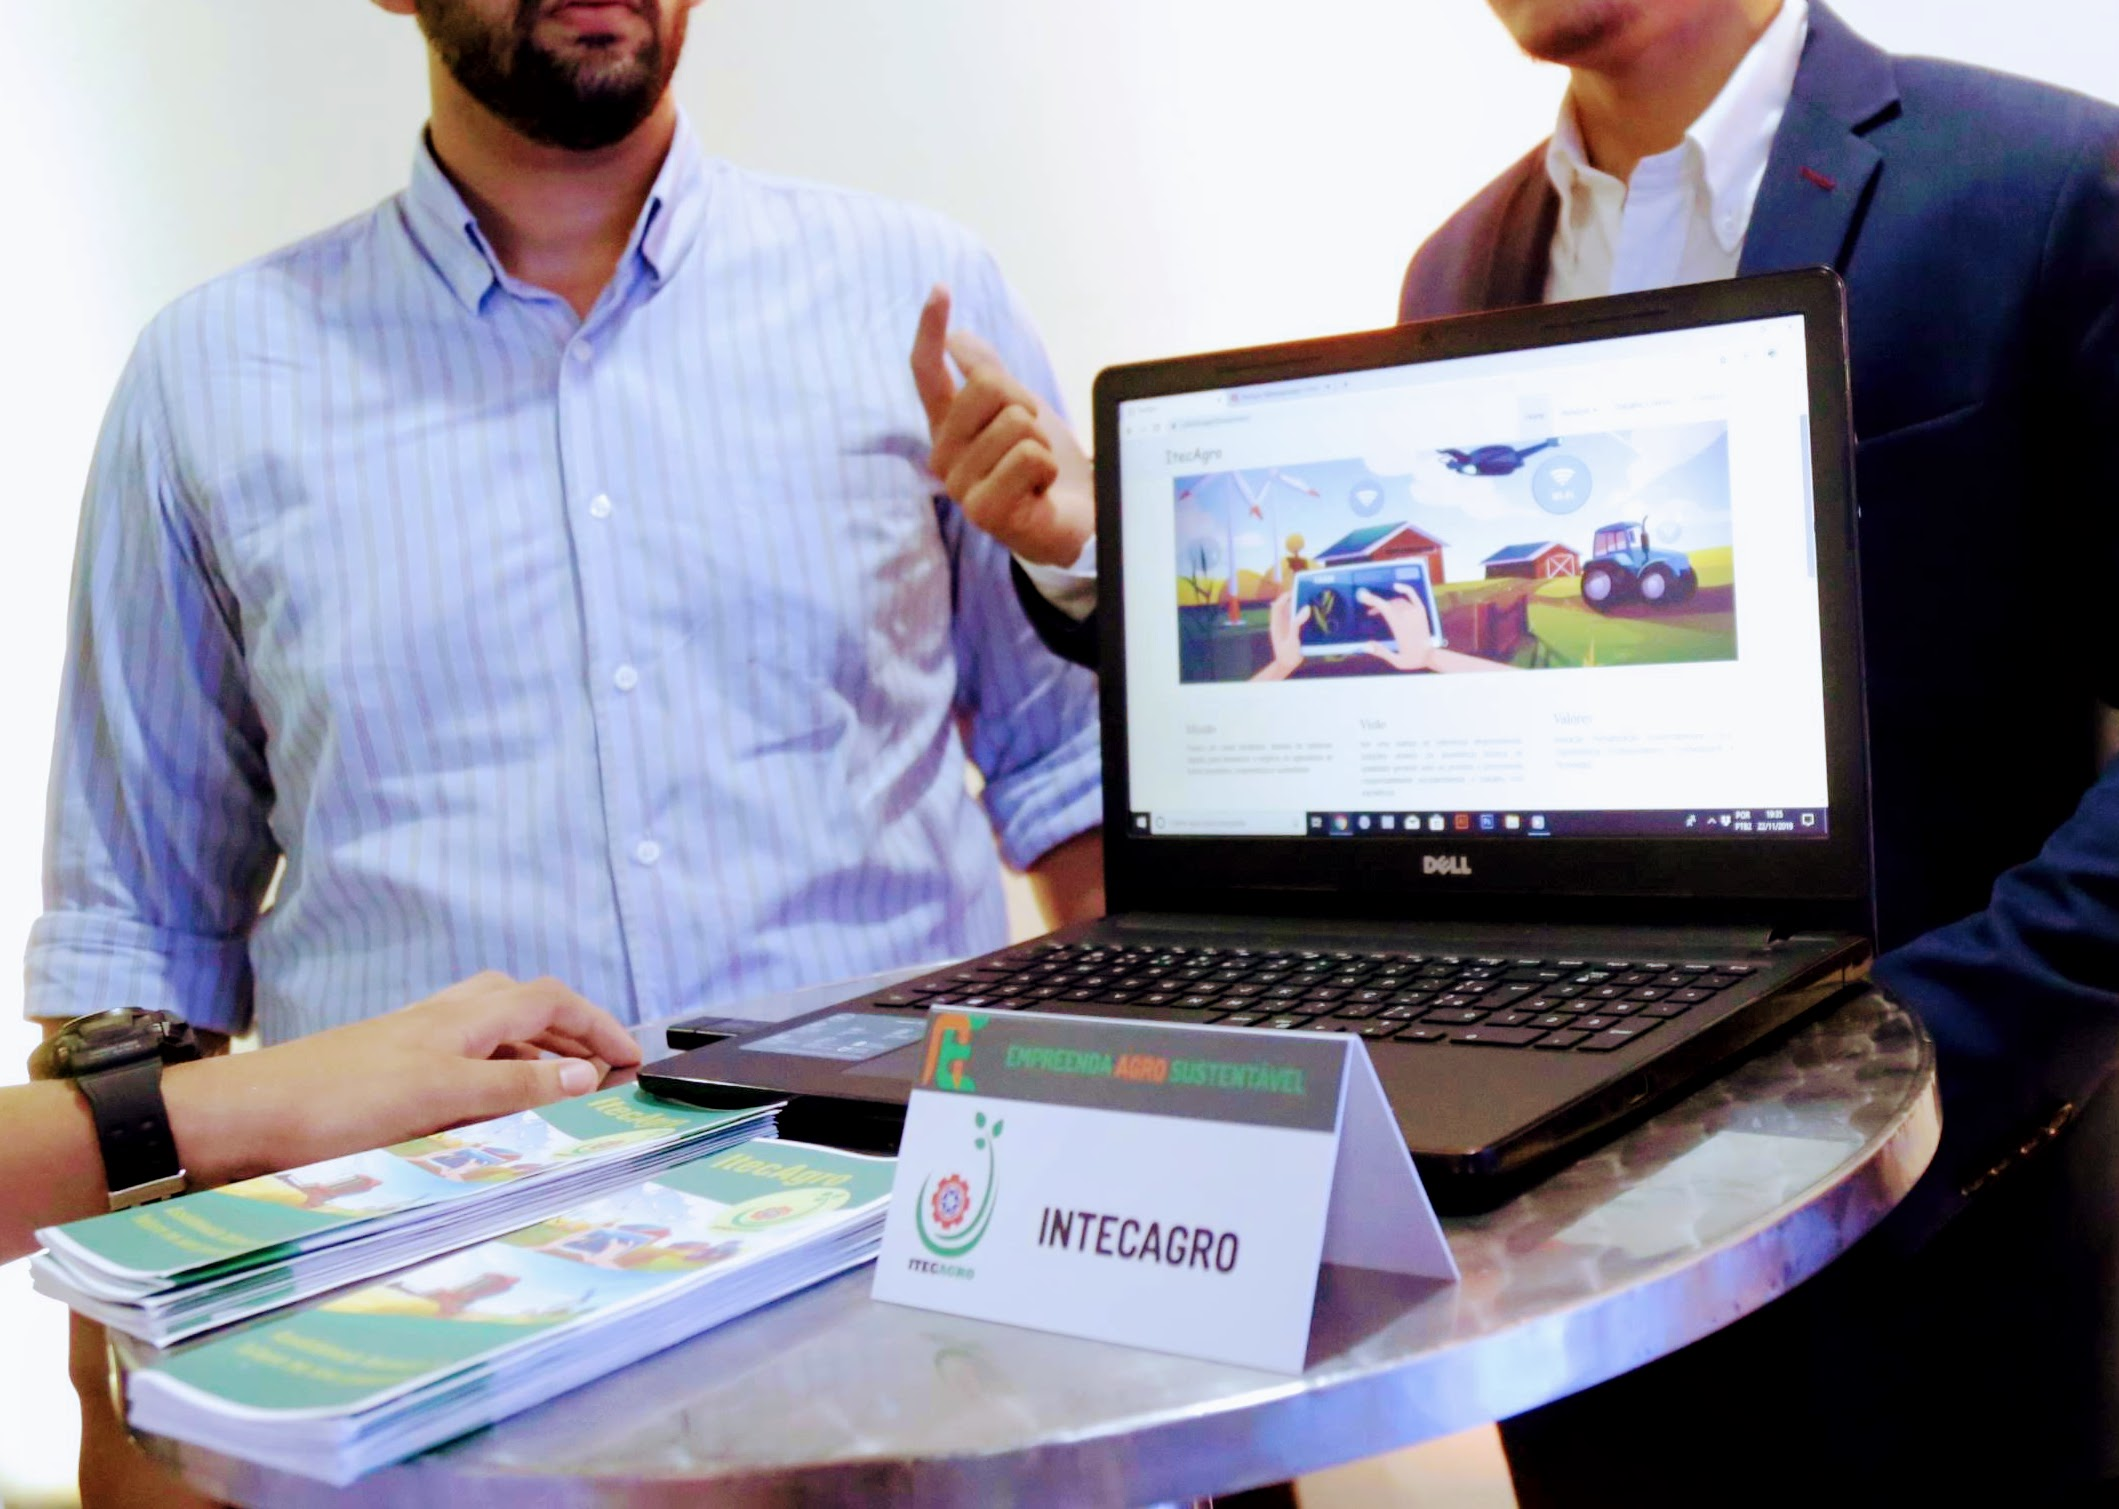
\includegraphics[scale=0.085]{Imagens/prototipo_5.jpg}}
\qquad
\subfigure[ref3][MCVP desenvolvido por Ranagro ]{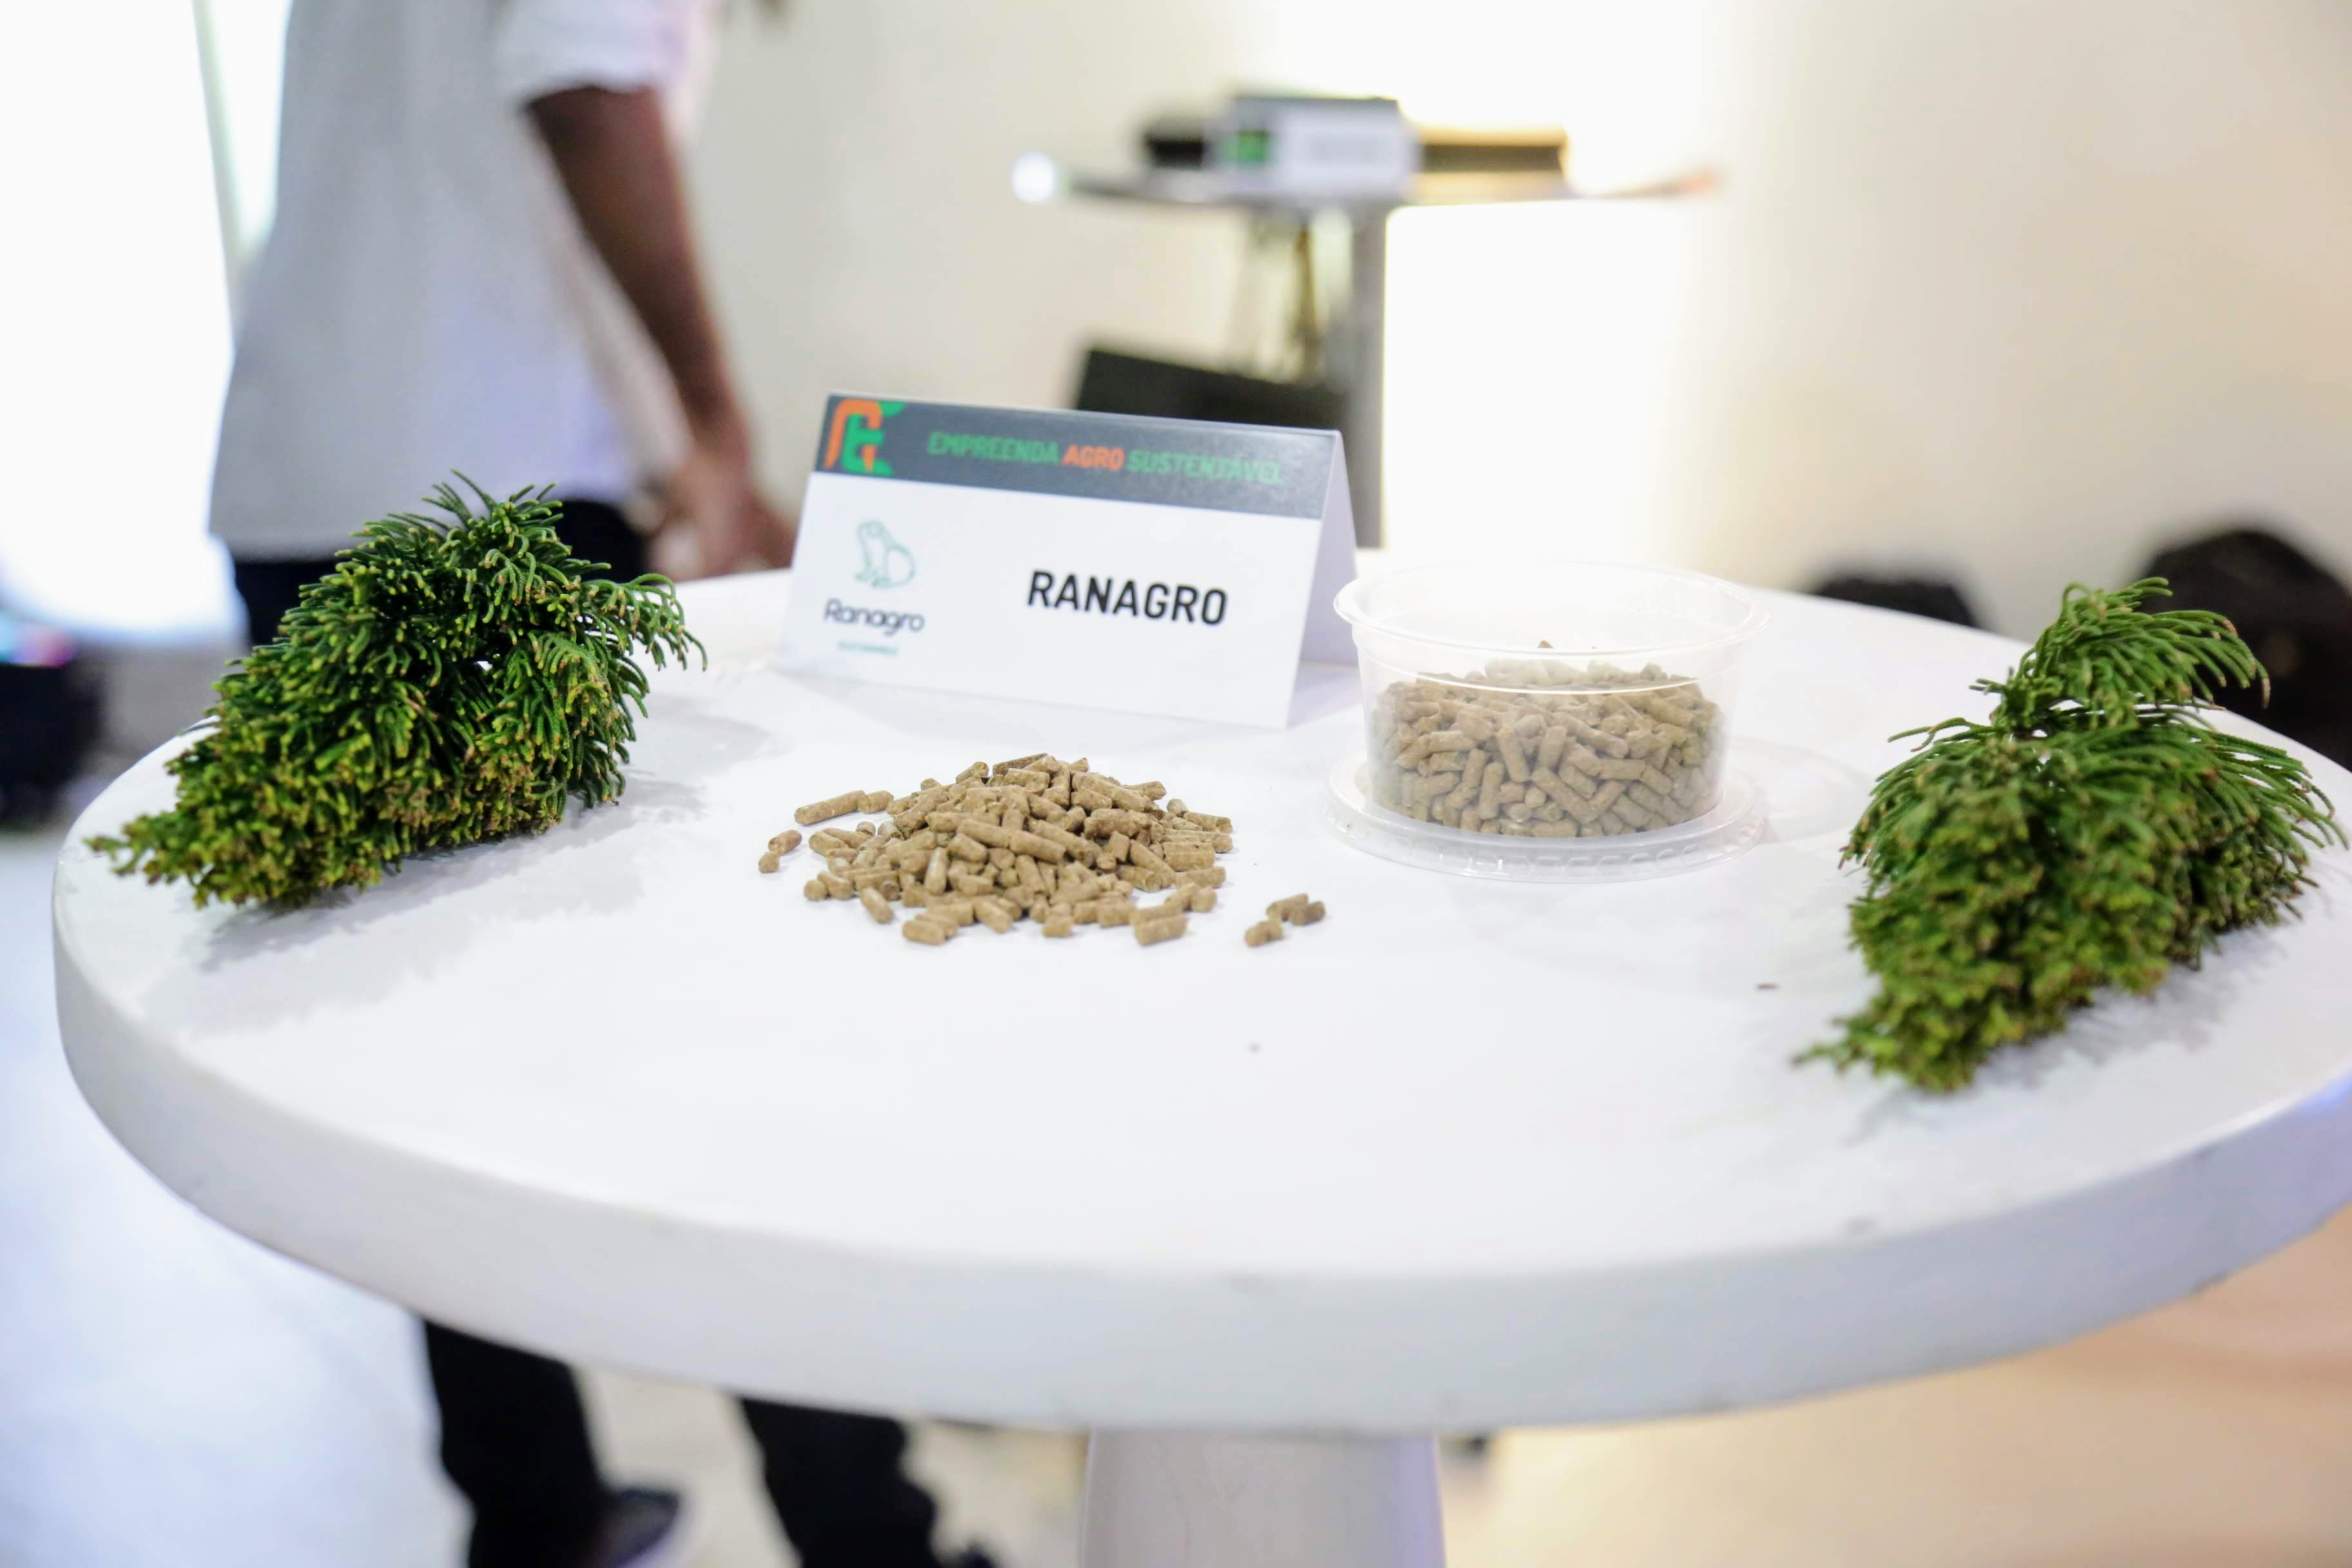
\includegraphics[scale=0.05]{Imagens/prototipo_6.jpg}}

\fonte{O Autor}.
\label{figura_mvp}
\end{figure}


\begin{landscape}
\label{app:portfolio}

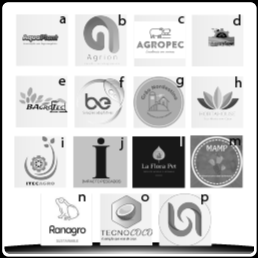
\includepdf[landscape=true,scale=0.70,pagecommand=\chapter{Portfólio Empreenda}]{apendece/portfolio.pdf}
\end{landscape}
\includepdf[landscape=true,scale=0.80,pages={2-66},nup=2x2,pagecommand={}]{apendece/portfolio_pb.pdf}

% ----------------------------------------------------------
\end{apendicesenv}
